\chapter{Evaluation de l'efficacité du Neurofeedback par la méta-analyse} \label{chapitre-2}

\section*{Introduction}
Les méta-analyses ont pour but de combiner les données de plusieurs études visant à démontrer l'efficacité d'un traitement. Cette méthode est
particulièrement intéressante lorsque les études comportent un faible nombre de sujets ou que les résultats des études se contredisent, 
comme c'est notamment le cas pour le \gls{nfb} appliqué aux enfants \gls{tdah}, qui est l'un des principaux usages du \gls{nfb}. 

Les différentes étapes à suivre pour réaliser une méta-analyse sont détaillées précisément dans ce chapitre.
Ces étapes sont ensuite appliquées à la réplication et à la mise à jour d'une récente méta-analyse sur l'efficacité du \gls{nfb} appliqué aux enfants 
souffrant de \gls{tdah} :
celle de \citet{Cortese2016} dont certains résultats ont été débattus par la communauté scientifique \citep{Micoulaud2016}. Ainsi, cette analyse a pour but
de relever l'éventuel impact de certains choix méthodologiques de \citet{Cortese2016} sur ses conclusions quant à l'efficacité du \gls{nfb} et de mettre à jour
ces résultats en incluant de nouvelles études. 

A travers le travail présenté ici, la performance du \gls{nfb} sur les enfants \gls{tdah} est alors évaluée et la revue de littérature
qui a été menée a permis de se familiariser avec les études sur l'efficacité de ce traitement et d'en noter les éventuelles faiblesses.

\newpage

\section{Principe d'une méta-analyse} \label{methods}

Les différentes étapes pour réaliser une méta-analyse sont décrites dans cette partie et résumées à la Figure~\ref{Figure:pipeline_meta_analyse}. 
Bien qu'il existe des logiciels permettant de réaliser une méta-analyse, ces étapes ont été implémentées en Python par souci de transparence et de reproductibilité. 
En effet, les logiciels généralement employés proposent une interface graphique où les formules mathématiques utilisées ne sont pas énoncées clairement. Le code source de ce package 
Python est disponible sur un dépôt GitHub \citep{Bussalb2019clinical} avec sa documentation associée générée par Sphinx (version 1.5.6.).

\subsection{Buts d'une méta-analyse}

Les méta-analyses rassemblent les résultats de plusieurs études, satisfaisant des critères d'inclusion préalablement établis, dans le but d'analyser
sur un plus grand nombre de sujets provenant de populations différentes, l'efficacité d'un traitement. 

\begin{figure}[h!]
  \centering
	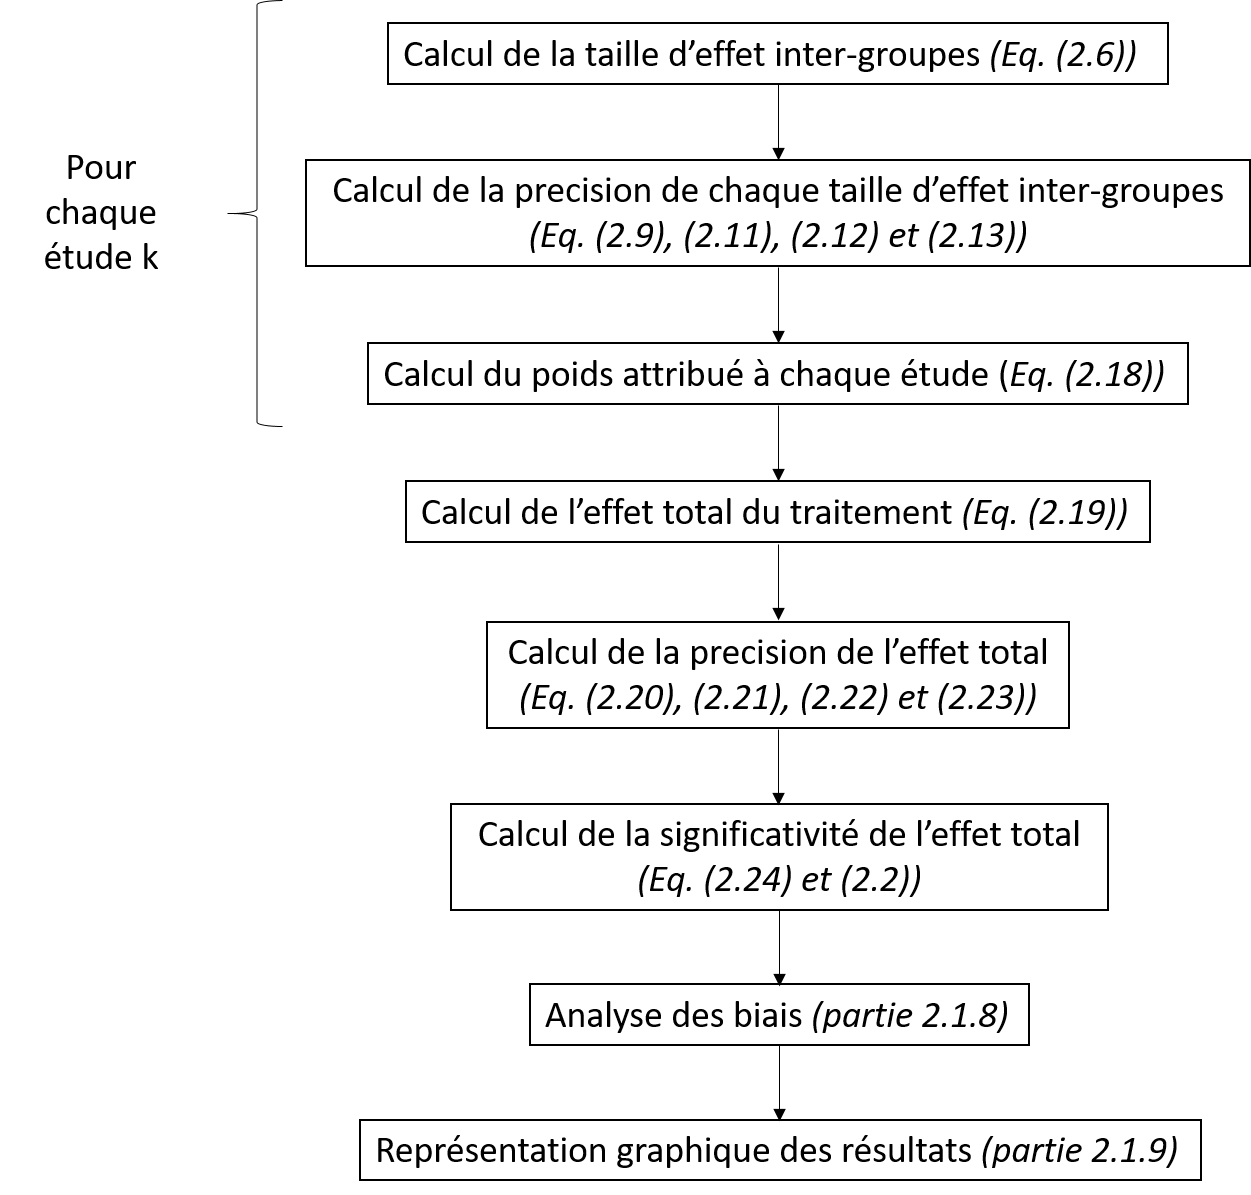
\includegraphics[width=1.0\linewidth]{figures/chapter-2/pipeline-perform-meta-analysis} 
  \caption[Résumé des étapes d'une méta-analyse.]{Résumé des étapes à suivre pour effectuer une méta-analyse dans le cadre d'un modèle à effets aléatoires.}
  \label{Figure:pipeline_meta_analyse}
\end{figure}

Alors qu'avant les années 1990 les revues narratives (\textit{narrative reviews} en anglais) étaient le plus couramment utilisées pour cette tâche, elles ont 
perdu leur popularité au profit des méta-analyses. En effet, les revues narratives souffrent de la subjectivité des auteurs qui choisissent notamment le poids 
à donner à telle ou telle étude : alors que certains
vont donner plus d'importance aux études incluant de nombreux sujets, d'autres vont favoriser celles qu'ils jugent de bonne qualité. La méta-analyse permet 
de réduire cette subjectivité en utilisant par exemple des critères mathématiques définis à l'avance pour calculer le poids à attribuer à chaque étude incluse
\citep[Chapitre~1]{Borenstein2009}. 

Par ailleurs, des recommandations précises quant à la conduite d'une méta-analyse existent \citep{Moher2009, Cochrane}. Ces recommandations
appellent notamment à apporter un soin particulier à la sélection des études qui doivent répondre à des critères d'inclusion fixés 
\textit{a priori} et à évaluer le risque de biais intra et inter-études, comme le biais de publication \citep{Higgins2011}. Ce biais consiste, 
pour un chercheur, à avoir tendance à publier des expériences présentant des résultats statistiquement significatifs.  

Réaliser une méta-analyse permet de confronter les résultats de toute étude incluse à ceux des autres études intégrées dans l'analyse.
L'efficacité du traitement observée pour chaque étude est mesurée à l'aide d'une valeur appelée taille 
d'effet (ou \gls{es} en anglais) présentée en \ref{definition_es} qui est, le plus souvent, standardisée du fait du regroupement de 
populations et de mesures relativement hétérogènes \citep{Cortese2016}.

\subsection{Choix du modèle} \label{model_choice}

La première étape consiste à choisir le modèle statistique de la méta-analyse. La plupart des méta-analyses sont basées sur l'un des deux modèles 
suivants qui reposent sur des hypothèses scientifiques différentes \citep[Chapitre~10]{Borenstein2009} :
\begin{itemize}
\item le modèle à effet fixe (\textit{fixed-effect model} en anglais),
\item le modèle à effets aléatoires (\textit{random-effects model} en anglais).
\end{itemize}

Dans le cas du modèle à effet fixe, il est supposé qu'il existe un \gls{es} réel (\textit{true} \gls{es} en anglais), c'est à dire l'\gls{es} qui serait
observé avec un nombre de sujets infiniment grand, qui serait le même pour l'ensemble des études incluses dans la méta-analyse. Les différences entre
les \gls{es} observés pour chaque étude sont dues à des erreurs d'échantillonnage. Au contraire, dans le cas du modèle à effets aléatoires, 
l'\gls{es} réel peut varier entre les études. Cette variabilité s'explique non seulement par des erreurs d'échantillonnage, mais aussi par 
les différentes conceptions des études et/ou par les différences entre les sujets inclus.

Les \gls{es} obtenus pour chaque étude sont moyennés pour mener à un \gls{est} (\textit{summary effect} en anglais dont le calcul est
décrit en \ref{compute_summary_effect}) sur lequel une hypothèse nulle est testée, qui diffère selon le modèle choisi :
\begin{itemize}
\item pour le modèle à effet fixe : 
\textit{$H_{0}$ : le traitement n'a auncun effet dans chaque étude},
\item pour le modèle à effets aléatoires : 
\textit{$H_{0}$ : l'effet moyen du traitement est nul}.
\end{itemize}

Le modèle à effets aléatoires est souvent plus approprié du fait de la variabilité des études. En effet, même si les études incluses dans la méta-analyse 
répondent toutes aux critères d'inclusion fixés au préalable, rien ne peut généralement permettre de supposer que ces études sont identiques et qu'elles 
partagent donc toutes le même \gls{es} réel. Le modèle à effet fixe est ainsi rarement utilisé, on peut cependant y avoir recours lorsque le nombre d'études incluses 
est très petit. En effet, dans le cas du modèle à effet fixe, les poids associés à chaque étude sont moins équilibrés : les études incluant un grand nombre de 
sujets se voient attribuer un poids plus important que dans le cas du modèle à effets aléatoires, et les études aux petits échantillons un plus faible poids.

Au sein du domaine du \gls{nfb} appliqué aux enfants \gls{tdah}, les méta-analyses suivent le modèle à effets aléatoires 
\citep{Cortese2016, Micoulaud2014}. Ainsi, étant donné l'hétérogénéité des populations étudiées et des critères d'évaluation, et pour être en accord avec
la littérature existante, c'est le modèle à effets aléatoires qui est utilisé par la suite.

\subsection{Calcul de la taille d'effet} \label{definition_es}

Une fois le modèle choisi, l'étape suivante est de quantifier l'efficacité de chaque étude incluse dans la méta-analyse en calculant son \gls{es}. 
Il existe différents \gls{es} \citep[Chapitre~3]{Borenstein2009} :
\begin{itemize}
\item \gls{es} basés sur des \emph{moyennes} :
\begin{itemize}
    \item la différence moyenne non standardisée (\textit{unstandardized mean difference} en anglais), D :
		    \begin{equation}
        \label{eq:metareview_unstandardized_mean_difference}
        \text{D} = \mu_{1} - \mu_{1},
        \end{equation} 
		avec $\mu_{1}$ et $\mu_{2}$ les moyennes de deux groupes indépendants, ou du même groupe à pré- et à post-test,
    \item la différence moyenne standardisée (\textit{standardized mean difference} en anglais), d :
		    \begin{equation}
        \label{eq:metareview_standardized_mean_difference}
        \text{d} = \frac{\mu_{1} - \mu_{2}}{\sqrt{\frac{(n_1 - 1)\sigma_1^2 + (n_2 - 1)\sigma_2^2} {n_1 + n_2 - 2}}},
        \end{equation} 
		avec $n_{1}$ et $n_{2}$ le nombre de sujets dans les groupes 1 et 2, et $\sigma_{1}$ et $\sigma_{2}$ les écarts-types des deux groupes. Le dénominateur
		correspond à l'écart type intra-groupe calculé à travers les deux groupes.
\end{itemize}
\item \gls{es} basés sur des \emph{données binaires} :
\begin{itemize}
    \item le taux de risque (\textit{risk ratio} en anglais), RR :
				\begin{equation}
        \label{eq:metareview_risk_ratio}
        \text{RR} = \frac{ \text{A} / n_1 } { \text{C} / n_2 },
        \end{equation} 
		avec A et C le nombre d'évènements observés (par exemple présence d'un effet secondaire) respectivement dans les groupes 1 et 2,
    \item le taux de chance (\textit{odds ratio} en anglais), OR :
				\begin{equation}
        \label{eq:metareview_odds_ratio}
        \text{OR} = \frac{ \text{AD} } { \text{BC} },
        \end{equation} 		
		avec D et B le nombre de non-évènements observés (par exemple absence d'un effet secondaire) respectivement dans les groupes 2 et 1,
		\item la différence de risque (\textit{risk difference} en anglais), RD :
				\begin{equation}
        \label{eq:metareview_risk_difference}
        \text{RD} = \frac{ \text{A} } { n_1 } - \frac{ \text{C} } { n_2 }.
        \end{equation}
\end{itemize}
\end{itemize}

Etant donné que les données que nous allons utiliser pour la réplication et la mise à jour de \citet{Cortese2016} sont les moyennes des 
scores cliniques obtenus par les sujets sur des échelles évaluant les symptômes du \gls{tdah} avant le traitement (pré-test) et 
après le traitement (post-test) et leur écart-type, nous nous concentrons sur 
les \gls{es} basés sur des moyennes. Par ailleurs, les échelles cliniques variant 
d'une étude à l'autre, les moyennes et les écarts-types ne sont pas comparables : il faut donc standardiser l'\gls{es}. 
Ainsi, nous allons utiliser la différence moyenne standardisée \citep{Cortese2016, Micoulaud2014}.

Enfin, lorsqu'un groupe contrôle est disponible, on peut calculer l'\gls{es}-inter-groupes (\textit{between}-\gls{es} en anglais) comme défini par \citet{Morris2008}.
Cet \gls{es} est utilisé par \citet{Cortese2016} et \citet{Micoulaud2014} et implémenté dans \citet{Bussalb2019clinical} :
\begin{equation}
\label{eq:metareview_effect_size_between}
\text{ES-inter-groupes} = c_p \left(\frac{(M_{\text{post},T} - M_{\text{pré},T}) - (M_{\text{post},C} - M_{\text{pré},C}) }{\sigma_{\text{pré}}} \right).
\end{equation} 

L'\gls{es}-inter-groupes est équivalent au $Z$-score d'une distribution normale qui est une mesure de combien d'écarts-types un score brut est au-dessus ou en-dessous
de la moyenne d'une population. 

L'\gls{es}-inter-groupes correspond à la différence entre la moyenne à post-test et à pré-test 
dans le groupe qui reçoit le traitement ($M_{\text{post},T}$, $M_{\text{pré},T}$) moins la différence entre la moyenne du score à post-test et à pré-test 
dans le groupe contrôle ($M_{\text{post},C}$, $M_{\text{pré},C}$), divisée par la \textit{pooled standard deviation} à pré-test ($\sigma_{\text{pré}}$) :
\begin{equation}
\label{eq:stats_metareview_std_pre}
\sigma_{\text{pré}} = \sqrt{\frac{(n_T - 1)\sigma_{\text{pré}, T}^2 + (n_C - 1)\sigma_{\text{pré}, C}^2} {n_T + n_C - 2}},
\end{equation}
où $\sigma_{\text{pré},G}$ correspond à l'écart-type du groupe $G$ à pré-test et $n_G$ indique le nombre de sujets ayant suivi l'intégralité 
du traitement dans chaque groupe.

La normalisation de l'\gls{es}-inter-groupes (équation Eq.~(\ref{eq:metareview_effect_size_between})) à l'aide de $\sigma_{\text{pré}}$ 
(équation Eq.~(\ref{eq:stats_metareview_std_pre})) se fait seulement avec les données obtenues en pré-test pour ne pas y inclure la variabilité 
induite par le traitement.

Il s'avère que l'\gls{es}-inter-groupes présente un léger biais qui tend à sous-estimer la valeur absolue de la différence moyenne standardisée de la population
lorsque les études incluent peu de sujets. Cette valeur est obtenue en calculant la différence entre les vraies moyennes de la population de chaque groupe divisée 
par l'erreur type de la vraie population qui est supposée être identique pour les deux groupes \citep[Chapitre~4]{Borenstein2009}. Ce biais peut être supprimé 
grâce à un facteur de correction $c_p$ qui est utilisé pour les petites études (c'est à dire pour lesquelles $n_T + n_C - 2 < 10$) : 
\begin{equation}
\label{eq:metareview_correction_factor}
c_p =  1 - \frac{3} {4(n_T + n_C - 2) - 1},
\end{equation} 
avec $n_T + n_C - 2$ qui correspond au dégré de liberté utilisé pour le calcul de $\sigma_{\text{pré}}$ à l'équation Eq.~(\ref{eq:stats_metareview_std_pre}).

Plus la valeur absolue de l'\gls{es}-inter-groupes est élevée, plus l'efficacité du traitement est importante. En effet, la valeur absolue d'un \gls{es}-inter-groupes 
se situant entre 0.2 et 0.5 rend compte d'une faible efficacité, une efficacité moyenne correspond à une valeur absolue entre 0.5 et 0.8, et lorsqu'elle est supérieure à 0.8 
l'efficacité du traitement est importante. Toutefois, l'interprétation de la valeur de l'\gls{es}-inter-groupes dépend du domaine d'application \citep{fritz2012}. Dans les
analyses qui suivent, un \gls{es}-inter-groupes négatif est en faveur du \gls{nfb}.  

\subsection{Calcul de la fiabilité de chaque taille d'effet}

Le terme précision englobe trois valeurs statistiques liées les unes aux autres : la variance, l'\gls{et} (à ne pas confondre avec
l'écart type), et l'intervalle de confiance.
Ces trois facteurs de précision définissent un intervalle de valeurs probables pour l'\gls{es} réel. 

Tout d'abord, la variance de chaque \gls{es}-inter-groupes est calculée \citep{Morris2008}:
\begin{equation}
\label{eq:metareview_variance_effect_size_between}
\sigma^2(\text{ES}) = c_p^2 \left(
    \frac{n_T + n_C - 2} {n_T + n_C - 4} 
\right ) \left ( 
		\frac{2(1-r)(n_T + n_C)} {n_Tn_C} + \text{ES}^2 
\right) - \text{ES}^2,
\end{equation}
où \gls{es} désigne l'\gls{es}-inter-groupes et $r$ la corrélation de Pearson groupée intra-groupes \citep{James2013} :
\begin{equation}
\label{eq:metareview_within_group_pearson_correlation}
r = \frac{ \sum_{i=1}^{n} (\text{s}_{\text{pré},i} - \mu_{\text{pré}})(\text{s}_{\text{post},i} - \mu_{\text{post}}) } { \sqrt{ \sum_{i=1}^{n} (\text{s}_{\text{pré},i} - 
\mu_{\text{pré}})^2} \sqrt{\sum_{i=1}^{n} (\text{s}_{\text{post},i} - \mu_{\text{post}})^2} }, 
\end{equation}
où $n$ est le nombre de patients inclus dans une étude, $\text{s}_{\text{pré},i}$, $\text{s}_{\text{post},i}$ les valeurs de scores cliniques pour le sujet $i$ 
respectivement à pré- et post-test, et $\mu_{\text{pre}}$, $\mu_{\text{post}}$ les scores moyens calculés sur tous les sujets. 
Il s'agit d'une mesure de corrélation linéaire entre deux variables : une valeur de 1 signifie une corrélation positive entre ces variables,
une valeur de -1 une corrélation négative, et une valeur de 0 une absence de corrélation linéaire. Ainsi, si le traitement n'a aucun effet, 
que l'état des sujets n'évolue pas naturellement, et en l'absence de bruit, $r$ sera égal à 1. On peut en déduire alors qu'une étude 
composée d'enfants plus jeunes qui sont davantage susceptibles de changer naturellement va présenter une valeur de $r$ plus faible, il en va 
de même si le traitement est efficace. Enfin la présence de bruit va également avoir un impact sur cette valeur. Par conséquent, une valeur 
de $r$ doit être calculée pour chaque étude.

Dans notre cas, cette corrélation étant inconnue et les données brutes n'étant pas disponibles pour la majorité des études cliniques, nous approximons la valeur 
de $r$ en accord avec \citet{Balk2012}, qui a trouvé qu'une valeur de 0.5 conduit à des résultats proches de ceux obtenus avec la véritable
valeur de la corrélation.

Une fois la variance obtenue, il est aisé de calculer l'\gls{et} (\textit{standard error} en anglais) de l'\gls{es}-inter-groupes \citep[Chapitre~8]{Borenstein2009} :
\begin{equation}
\label{eq:metareview_standard_error_effect_size_between}
\text{ET} = \sqrt{\sigma^2(\text{ES})} = \sigma(\text{ES}),
\end{equation}
où \gls{es} désigne l'\gls{es}-inter-groupes. Alors que la variance est intéressante pour les calculs statistiques, l'\gls{et} est quant à elle 
un index plus aisé à comprendre car elle est sur la même échelle que l'\gls{es}.

Enfin, si on suppose que l'\gls{es}-inter-groupes suit une distribution normale, son intervalle de confiance à 95\% peut être calculé \citep[Chapitre~8]{Borenstein2009} :
\begin{equation}
\label{eq:metareview_es_between_confidence_interval_95_lower_bound}
\text{LL} = \text{ES-inter-groupes} - 1.96 * \text{ET},
\end{equation}
et 
\begin{equation}
\label{eq:metareview_es_between_confidence_interval_95_upper_bound}
\text{UL} = \text{ES-inter-groupes} + 1.96 * \text{ET},
\end{equation}
où LL correspond à la limite inférieure de l'intervalle et UL à la limite supérieure. La valeur de 1.96 correspond au $Z$-score d'une distribution 
normale standard pour un intervalle de confiance à 95\%. La probabilité de trouver dans cet intervalle
la vraie valeur de l'\gls{es}-inter-groupes de la population est de 95\%.

La précision est affectée, dans une large mesure, par le nombre de sujets inclus dans l'étude : les échantillons plus grands mènent à des
variances plus faibles et donc à des estimations d'\gls{es}-inter-groupes plus précises \citep[Chapitre~8]{Borenstein2009}, c'est pourquoi un plus grand 
poids leur est attribué dans la méta-analyse comme détaillé par la suite.

\subsection{Calcul de la taille d'effet totale du traitement} \label{compute_summary_effect}

Afin d'obtenir l'estimation la plus précise possible de l'effet du traitement sur la population, une moyenne pondérée des \gls{es}-inter-groupes 
des études incluses est calculée.

Si le modèle à effet fixe est choisi, le poids $w_{\text{fixe},k}$ assigné à chaque étude $k$ correspond à l'inverse de la variance de son 
\gls{es}-inter-groupes ($\sigma^2(\text{ES})$, la variance intra-étude) \citep[Chapitre~12]{Borenstein2009} :
\begin{equation}
\label{eq:metareview_weight_fixed_study}
w_{\text{fixe},k} = \frac{1}{\sigma^2(\text{ES}_k)}.
\end{equation} 

Cette étape a pour but de minimiser l'importance des études avec une large variabilité intra-étude.

Dans notre cas nous employons le modèle à effets aléatoires, qui inclut également la variance inter-études $\tau^2$ conduisant à des 
poids $w_{\text{aléatoires},k}$, simplement notés $w_k$ par la suite, associés aux études différents.
Toutefois, afin d'obtenir les poids $w_k$, il est nécessaire de calculer d'abord les $w_{\text{fixe},k}$ grâce à l'équation 
Eq.~(\ref{eq:metareview_weight_fixed_study}).

Calculer la variance inter-études se fait en trois étapes décrites par les équations Eq.~(\ref{eq:metareview_Q}), Eq.~(\ref{eq:metareview_C}) 
et Eq.~(\ref{eq:metareview_Tau}) \citep[Chapitre~12]{Borenstein2009} :
\begin{equation}
\label{eq:metareview_Q}
Q = \sum_{k=1}^{K} w_{\text{fixe},k} * \text{ES}_k^2,
\end{equation}
\begin{equation}
\label{eq:metareview_C}
C = \sum_{k=1}^{K} w_{\text{fixe},k} - \frac{ \sum_{k=1}^{K} (w_{\text{fixe},k})^2 } { \sum_{k=1}^{K} w_{\text{fixe},k} },
\end{equation}
avec $K$ le nombre total d'études incluses, et :
\begin{equation}
\label{eq:metareview_Tau}
\tau^2 = \frac{Q - \text{df}}{C},
\end{equation}
avec $\text{df} = K - 1$ le degré de liberté.

Le modèle à effets aléatoires prenant en compte les différences entre les études, les poids sont égaux à l'inverse de la somme entre la variance intra-étude
$\sigma^2(\text{ES}_k)$ et la variance inter-études $\tau^2$ \citep[Chapitre~12]{Borenstein2009} :
\begin{equation}
\label{eq:metareview_weight_study}
w_k = \frac{1}{\sigma^2(\text{ES}_k) + \tau^2}.
\end{equation} 

Enfin, la moyenne pondérée des $K$ \gls{es}-inter-groupes est calculée pour obtenir l'\gls{est} comme décrit dans l'équation
Eq.~(\ref{eq:metareview_summary_effect}) \citep[Chapitre~12]{Borenstein2009}:
\begin{equation}
\label{eq:metareview_summary_effect}
\text{EST} = \frac{\sum_{k=1}^{K} w_k * \text{ES}_k} {\sum_{k=1}^{K} w_k}.
\end{equation} 

\subsection{Calcul de la fiabilité de la taille d'effet totale}

Une fois l'\gls{est} obtenu, on peut calculer ses trois valeurs de précision \citep[Chapitre~12]{Borenstein2009}. Tout d'abord, sa variance $\sigma^2(\text{EST})$ :  
\begin{equation}
\label{eq:metareview_variance_summary_effect}
\sigma^2(\text{EST}) = \frac{1} {\sum_{k=1}^{K} w_k},
\end{equation} 
puis son \gls{et} ET(EST) :
\begin{equation}
\label{eq:metareview_standard_error_effect}
\text{ET(EST)} = \sqrt{\sigma^2(\text{EST})} = \sigma(\text{EST}),
\end{equation} 
et enfin son intervalle de confiance à 95\% : 
\begin{equation}
\label{eq:metareview_confidence_interval_summary_effect_lower_bound}
\text{LL(EST)} = \text{EST} - 1.96 * \text{ET(EST)},
\end{equation}
et 
\begin{equation}
\label{eq:metareview_confidence_interval_summary_effect_upper_bound}
\text{UL(EST)} = \text{EST} + 1.96 * \text{ET(EST)},
\end{equation}
avec LL la limite inférieure de cet intervalle de confiance et UL sa limite supérieure.

\subsection{Calcul de la significativité statistique de la taille d'effet totale}

Une $Z$-value est calculée pour tester l'hypothèse nulle pour le modèle à effets aléatoires énoncée en \ref{model_choice} \citep[Chapitre~12]{Borenstein2009} :
\begin{equation}
\label{eq:metareview_confidence_interval_summary_effect_z_value}
Z = \frac{\text{EST}} {\text{ET(EST)}}.
\end{equation}

Pour un test bilatéral (utilisé par \citet{Micoulaud2014, Cortese2016}), la $p$-value est ensuite calculée avec \citep[Chapitre~12]{Borenstein2009} :
\begin{equation}
\label{eq:metareview_confidence_interval_summary_effect_p_value}
p = 2(1 - \Phi(\abs{Z})),
\end{equation} 
où $\Phi$ est la fonction de distribution cumulative de la loi normale standardisée (\textit{i.e.} centrée et normée).

Si la $p$-value obtenue est inférieure à 0.05, alors il y a une différence statistiquement significative entre l'efficacité du traitement étudié 
et celle du groupe contrôle.

D'autres valeurs peuvent ensuite être calculées pour compléter l'analyse, comme par exemple $I^2$ qui estime 
l'hétérogénéité des \gls{es}-inter-groupes \citep[Chapitre~16]{Borenstein2009}. 

\subsection{Analyse des biais}

Les résultats d'une méta-analyse peuvent être impactés par des biais, comme par exemple un biais de publication qui consiste en la tendance qu'ont les auteurs 
d'études scientifiques de plutôt publier des résultats statistiquement significatifs et en faveur de ce qu'ils veulent démontrer. De plus,
d'autres facteurs peuvent influencer les résultats de la méta-analyse : une faible qualité méthodologique conduisant à des effets faussement gonflés
dans les petites études, l'hétérogénéité des \gls{es} selon la taille des études, et le hasard \citep{Sterne2011}.

L'analyse visuelle de la symétrie d'un \textit{funnel plot} est une méthode couramment utilisée pour détecter un éventuel biais de publication et 
l'influence des facteurs cités précédemment \citep{Sterne2011}.

Il s'agit d'un nuage de points de la précision de chaque \gls{es}-inter-groupes en fonction des \gls{es}-inter-groupes. L'\gls{et} est couramment 
utilisée comme estimation de la précision et de la taille d'une étude et est placée sur un axe des abscisses inversé de façon à ce que les plus grandes études 
soient au sommet et que les plus petites se retrouvent 
dispersées en bas. En l'absence de biais et d'hétérogénéité entre les études, la répartition des points est seulement due à la variabilité de la taille des études : 
le graphique est symétrique. Le triangle centré sur l'\gls{est}, obtenu avec un modèle à effet fixe et s'étendant de 1.96 \gls{et} de chaque côté, 
inclut 95\% des études s'il n'y a pas de biais et si l'hypothèse du modèle à effet fixe est valide.

Déterminer l'asymétrie d'un \textit{funnel plot} peut se faire visuellement mais aussi mathématiquement en utilisant, par exemple, le test d'\citet{Egger1997}. 
Il s'agit de régresser les \gls{es}-inter-groupes divisés par leur \gls{et} sur l'inverse des \gls{et}. Si l'ordonnée à l'origine (\textit{intercept} en anglais) diffère significativement de 
zéro (seuil de significativité statistique à 5\%), alors le \textit{funnel plot} est asymétrique.

\subsection{Représentation graphique des résultats d'une méta-analyse}

Afin de faciliter la lecture des résultats d'une méta-analyse, ceux-ci sont résumés dans un \textit{forest plot} \citep[Chapitre~1]{Borenstein2009}. Les études incluses sont
en ordonnées et les \gls{es}-inter-groupes en abscisses. Chaque \gls{es}-inter-groupes est représenté par un carré dont la taille est proportionnelle
au poids $w_k$ attribué à l'étude $k$. Les intervalles de confiance à 95\% pour chaque \gls{es}-inter-groupes sont représentés. En bas du graphique, l'\gls{est}
est symbolisé par un diamant avec son intervalle de confiance à 95\%. Une droite verticale d'équation $x = 0$ est tracée pour délimiter la
partie du graphique où les \gls{es} sont en faveur du traitement de celle où ils ne le sont pas. Dans notre cas, la partie à gauche de cette droite (où les \gls{es}
sont négatifs) est en faveur du \gls{nfb}.

\section{Réplication et mise à jour de la méta-analyse de Cortese et al., 2016} 

La méta-analyse de \citet{Cortese2016} a eu un fort impact dans la communauté du \gls{nfb}, du fait du nombre d'études incluses (13) et 
du soin apporté à leur sélection. Cependant, certains choix méthodologiques ont fait l'objet de débats \citep{Micoulaud2016} et
méritent une attention particulière.
C'est pourquoi dans un premier temps, la méta-analyse de \citet{Cortese2016} est répliquée en modifiant les points débattus pour évaluer leur impact sur les
résultats. Ensuite, étant donné que la recherche dans le domaine du \gls{nfb} appliqué aux enfants \gls{tdah} est très active, de nouvelles études répondant au 
critère d'inclusion de \citet{Cortese2016} ont été publiées depuis cette méta-analyse. La mise à jour de ce genre d'analyse est importante
car plus des études y seront incluses, plus les résultats vont se stabiliser, c'est pourquoi la méta-analyse décrite en \ref{selection_studies}
comprend, en plus des 13 études originelles, celles qui
satisfont les critères d'inclusion de \citet{Cortese2016} depuis sa publication.

Dans un souci de transparence et pour faciliter la réplication de ce travail, ces deux analyses sont effectuées en utilisant le package Python 
(version de Python 3.6.1) dont le contenu est décrit en \ref{methods} \citep{Bussalb2019c}. Par conséquent, la première étape est d'évaluer la
fiabilité des résultats obtenus avec ce package.

\subsection{Evaluation des résultats obtenus avec le package Python} 

Pour effectuer une méta-analyse, les auteurs utilisent en général le logiciel RevMan \citep{Revman, Cortese2016, Micoulaud2014}. Ici, les résultats 
obtenus avec le package Python vont être comparés à ceux donnés par la version 5.1 de RevMan, présentés dans \citet{Cortese2016}, 
afin de valider l'utilisation de ce package.

\subsubsection{Matériel et méthodes}
La première étape a été d'entrer dans un fichier \gls{csv}, pour chaque étude incluse, les moyennes des scores cliniques à pré-test et post-test avec leur écart-type 
utilisés par \citet{Cortese2016} pour calculer les \gls{es}-inter-groupes. Lorsqu'ils sont disponibles, les scores cliniques évaluant l'inattention, l'hyperactivité 
et la totalité des symptômes sont extraits afin d'obtenir une valeur d'efficacité pour chacune de ces composantes. Par ailleurs, les scores donnés par les
parents (\gls{mprox}) mais aussi par les enseignants (\gls{pblind}) sont utilisés.

Une fois cette étape remplie, le package Python lit ce fichier et retourne l'\gls{est} ainsi que sa $p$-value associée en suivant les étapes présentées en
\ref{methods}, ce qui permet de conclure quant à l'efficacité du \gls{nfb} sur chaque composante.

\subsubsection{Résultats}
En accord avec les résultats de précédentes méta-analyses \citep{Sonuga-Barke2013, Micoulaud2014}, \citet{Cortese2016}
met en évidence un effet significativement favorable du \gls{nfb} lorsque son efficacité est calculée grâce aux évaluations des parents, mais aucune amélioration 
significative des symptômes n'est reportée par les enseignants. Ces résultats sont retrouvés lorsque l'analyse est effectuée par le programme Python, les valeurs
d'\gls{est} et leur $p$-value obtenues sont très proches voire égales à celles de \citet{Cortese2016} comme résumé dans la 
Table~\ref{Table:table_meta_review_comparison_revman_python}. 

\begin{table}[h!]
  \centering
  \caption[Comparaison entre les résultats de \citet{Cortese2016} obtenus avec RevMan \citep{Revman} et ceux obtenus avec le package Python.]{Comparaison entre les résultats de \citet{Cortese2016} obtenus avec RevMan \citep{Revman} et ceux obtenus avec le package Python \citep{Bussalb2019clinical}.
	Avec le package Python, un \gls{es} négatif est en faveur du \gls{nfb}. Le seuil de significativité statistique est fixé à 5\%.}
  \begin{tabular}{cccc}
\toprule

\multicolumn{2}{c}{Données} & \shortstack{ Resultats de \\ \citet{Cortese2016} } & \shortstack{ Résultats de \\ \citet{Bussalb2019clinical} } \\
\hline
\multicolumn{2}{c}{Implémentation} & \shortstack{ RevMan } & Package \textit{meta-analysis} \\
\hline
\multirow{3}{*}{ \textit{Parents} } & Total & $0.35$ ($0.004$) & $-0.34$ ($0.004$)\\
 & Inattention  & $0.36$ ($0.009$) & $-0.35$ ($0.011$)\\
 & Hyperactivité  & $0.26$ ($0.004$) & $-0.24$ ($0.02$)\\
\midrule
\multirow{3}{*}{ \textit{Enseignants} } & Total & $0.15$ ($0.20$) & $-0.13$ ($0.25$)\\
 & Inattention  & $0.06$ ($0.70$) & $-0.09$ ($0.50$)\\
 & Hyperactivité  & $0.17$ ($0.13$) & $-0.15$ ($0.21$)\\
\bottomrule
\end{tabular}

  \label{Table:table_meta_review_comparison_revman_python}
\end{table}

Les différences de signe entre les \gls{est} de \citet{Cortese2016} et ceux de \citet{Bussalb2019clinical} s'expliquent par le choix qu'il a été fait de ne pas multiplier
par -1 les \gls{es}-inter-groupes calculés avec l'équation Eq.~(\ref{eq:metareview_effect_size_between}), cette décision a également été prise par 
\citet{Micoulaud2014}.

Les petites différences observées notamment au niveau des $p$-values sont dues à notre décision d'utiliser systématiquement une corrélation de Pearson groupée intra-groupes
toujours égale à 0.5 \citep{Balk2012} lors du calcul de la variance de chaque \gls{es}-inter-groupes à l'équation 
Eq.~(\ref{eq:metareview_variance_effect_size_between}). Une analyse de sensibilité a été menée pour s'assurer de l'impact mineur de la valeur de la corrélation de Pearson groupée 
intra-groupes : lorsqu'elle varie entre 0.2 et 0.8, la significativité statistique de l'\gls{est} ne change pas.

Au vu de la faible différence entre ce qui est retourné par RevMan et par le package Python, la validité de ce dernier est confirmée : il sera donc utilisé pour mener
les analyses suivantes.

\subsection{Réplication de la méta-analyse de Cortese et al., 2016} \label{replication}

Certains choix de la méta-analyse de \citet{Cortese2016} ont été discutés par la communauté scientifique \citep{Micoulaud2016}. Le but de cette section est 
d'étudier leur impact sur les conclusions de cette méta-analyse.

\subsubsection{Materiel et méthodes}
Les changements suivants ont été mis en place afin d'être étudiés :

\begin{itemize}
\item l'\gls{es}-inter-groupes de \citet{Arnold2014} est calculé en utilisant les valeurs cliniques à post-test, c'est à dire obtenues lorsque la totalité 
des 40 sessions est effectuée, à la différence de \citet{Cortese2016} qui a utilisé les scores cliniques donnés apres 12 sessions de \gls{nfb} car les valeurs 
finales n'étaient pas encore disponibles,
\item \citet{Cortese2016} a calculé les \gls{es}-inter-groupes de \citet{Steiner2014} pour les enseignants à partir de leurs évaluations reportées sur 
la BOSS Classroom Observation \citep{Shapiro2010}. Ce choix interpelle car il s'agit d'une échelle peu commune pour quantifier les symptômes du \gls{tdah}, d'autant qu'une échelle clinique 
plus connue et bien définie \citep{Collett2003, Epstein2012, Bluschke2016}, la Conners-3 Teachers \citep{Conners1998, Conners2008}, est disponible dans 
cette étude. Ainsi, nous avons utilisé les scores cliniques donnés par les enseignants sur la Conners-3, échelle 
qui a d'ailleurs été utilisée pour calculer l'\gls{es}-inter-groupes basé sur l'évaluation des parents dans cette étude. 
\end{itemize}

\subsubsection{Résultats}

Les résultats obtenus avec ces changements sont résumés dans la Table~\ref{Table:table_meta_review_comparison_replication_cortese}.
La significativité statistique des \gls{est} est inchangée aussi bien pour les parents que pour les enseignants. Les variations de $p$-values sont expliquées
par le fait que les données de départ utilisées sont différentes de celles de \citet{Cortese2016} compte tenu des choix suivis ici.

\begin{table}[h!]
  \centering
  \caption[Comparaison entre les résultats de \citet{Cortese2016} et ceux de la réplication avec nos choix de modifications.]{Comparaison entre les résultats de \citet{Cortese2016} obtenus avec RevMan \citep{Revman} et ceux obtenus avec le package Python \citep{Bussalb2019clinical}
	avec nos choix de modifications ($^a$ valeurs à post-test de \citet{Arnold2014} sont prises après 40 sessions de \gls{nfb} et l'efficacité du \gls{nfb} évaluée 
	par les enseignants dans \citet{Steiner2014} se base sur la Conners-3 Teachers).
	Avec le package Python, un \gls{es} négatif est en faveur du \gls{nfb}. Le seuil de significativité statistique est fixé à 5\%.}
  \begin{tabular}{cccc}

\toprule
\multicolumn{2}{ c }{Hypothèses de travail} & \shortstack{ Celles de \\ \citet{Cortese2016} } & \shortstack{ Celles de \\ \citet{Bussalb2019a}$^a$ }\\
\midrule
\multirow{ 3}{*}{ \textit{Parents} } & Total & $0.35$ ($0.004$) & $-0.32$ ($0.013$)\\
 & Inattention  & $0.36$ ($0.009$) & $-0.31$ ($0.036$)\\
 & Hyperactivité  & $0.26$ ($0.004$) & $-0.24$ ($0.02$)\\
\midrule
\multirow{ 3}{*}{ \textit{Enseignants} } & Total & $0.15$ ($0.20$) & $-0.11$ ($0.37$)\\
 & Inattention  & $0.06$ ($0.70$) & $-0.17$ ($0.16$)\\
 & Hyperactivité  & $0.17$ ($0.13$) & $-0.022$ ($0.85$)\\
\bottomrule

\end{tabular}
  \label{Table:table_meta_review_comparison_replication_cortese}
\end{table}

L'influence de ces changements est examinée plus précisément en s'intéressant à leur impact individuel :
\begin{itemize}
\item les \gls{es}-inter-groupes obtenus pour l'étude de \citet{Arnold2014} après 40 sessions de \gls{nfb} sont plus faibles que ceux obtenus 
par \citet{Cortese2016}. Ces \gls{es}-inter-groupes plus faibles vont légèrement diminuer les \gls{est} mais sans impacter leur significativité statistique 
(cf. les trois premières lignes de la Table~\ref{Table:table_meta_review_comparison_replication_cortese}),
\item le calcul des \gls{es}-inter-groupes basé sur les évaluations des enseignants dans \citet{Steiner2014} avec la Conners-3 Teachers
conduit à un \gls{es}-inter-groupes plus élevé pour la composante inattention, mais plus faible pour les composantes hyperactivité et totale. Toutefois, ces
différences n'influencent pas la significativité statistique des \gls{est} (cf. les trois dernières lignes de la 
Table~\ref{Table:table_meta_review_comparison_replication_cortese}). 
\end{itemize}

Par conséquent, bien que ces points aient été débattus, leur impact sur les conclusions de la méta-analyse sont minimes et ne changent la significativité statistique 
d'aucun \gls{est}. 

\subsection{Mise à jour de la méta-analyse de Cortese et al., 2016} \label{selection_studies}

L'étape suivante consiste à mettre à jour la méta-analyse de \citet{Cortese2016} avec les choix faits lors de la réplication décrite en \ref{replication}. 
Pour ce faire, une recherche sur PubMed a été effectuée puis la performance du \gls{nfb} a été évaluée d'abord sur l'ensemble des études et ensuite sur 
des sous-groupes (un qui regroupe les études suivant un protocole standard \citep{Arns2014} et un autre qui comprend celles où les enfants se voient interdire la prise
de psychostimulants durant le traitement par \gls{nfb}) comme ce qui a été réalisé dans \citet{Cortese2016}. Ces analyses sont effectuées avec les choix définis en \ref{replication}.

\subsubsection{Matériel et méthodes}
Un soin particulier a été mis en oeuvre par \citet{Cortese2016} pour sélectionner les études bien conduites. Les principaux critères d'inclusion
et d'exclusion sont \citep{Cortese2016} :
\begin{itemize}
\item seules les études randomisées et contrôlées sont retenues,
\item les participants doivent avoir entre 3 et 18 ans et être diagnostiqués \gls{tdah},
\item les participants présentant une comorbidité rare sont exclus,
\item les contrôles acceptés sont : le traitement habituel, la liste d'attente, un traitement actif ou un placebo/\textit{sham}-\gls{nfb},
\item les études comparant le \gls{nfb} au traitement médicamenteux dont la dose est optimisée ou bien où le \gls{nfb} est couplé au traitement médicamenteux
dont la dose est optimisée sont exclues,
\item la prise de médicaments en tant que traitement en arrière-plan dans le groupe \gls{nfb} ou contrôle est acceptée.
\end{itemize}

Afin de trouver les études à inclure, \citet{Cortese2016} ont cherché sur plusieurs bases de données (dont la dernière vérification
date du 30 août 2015) telles qu'ERIC, OVID et PubMed. Dans notre cas seule PubMed, qui est la principale base de données, a été questionnée en entrant 
les mêmes termes de recherche que \citet{Cortese2016} (disponibles dans le matériel supplémentaire de leur méta-analyse).

La mise à jour de \citet{Cortese2016} se fait dans un premier temps avec l'ensemble des études (celles initialement incluses et celles nouvellement
identifiées), puis sur des sous-groupes.

La première sous-population étudiée correspond aux sujets ayant suivi un entraînement par \gls{nfb} dit \emph{standard}, c'est à dire répondant aux critères 
établis par \citet{Arns2014} :
\begin{itemize}
\item le protocole de \gls{nfb} utilisé a fait l'objet de plusieurs études cliniques (diminution du \gls{tbr}, augmentation du \gls{smr} et \gls{scp}),
\item une phase de transfert doit être proposée durant l'entraînement pour aider la transposition dans la vie de tous les jours,
\item le lieu où sont effectuées les sessions doit être précisé,
\item le traitement par \gls{nfb} doit satisfaire les critères de la théorie de l'apprentissage, c'est à dire ne pas utiliser de seuil de récompense automatique.
\end{itemize}

La deuxième sous-population étudiée comprend les sujets ne prenant aucun traitement médicamenteux durant le traitement par \gls{nfb}.

\subsubsection{Résultats de la sélection des études}

Finalement, 7 études ont été identifiées lors de la recherche menée le 2 septembre 2019, dont le détail est présenté 
à la Table~\ref{Table:table_meta_review_update_september_2019} : 
\begin{itemize}
\item \citet{Baumeister2016} pour qui seuls les résultats pour les symptômes totaux évalués par les parents sont disponibles,
\item \citet{Strehl2017} pour qui les évaluations des parents et des enseignants sont données pour toutes les composantes,
\item \citet{Bazanova2018} qui donne les évaluations des parents pour les composantes inattention, hyperactivité et totale (pour être cohérent avec 
la \gls{saob} présentée dans le chapitre \ref{ch-saob}, seul le groupe \gls{nfb} est retenu),
\item \citet{Minder2018} pour qui les évaluations des parents et des enseignants sont données pour toutes les composantes ; un groupe \gls{nfb}
et un groupe contrôle suivent leur traitement à l'école, alors que les autres groupes \gls{nfb} et contrôle l'effectue en clinique,
\item \citet{Moreno2019} pour qui seuls les résultats pour les symptômes totaux évalués par les parents sont disponibles,
\item \citet{Shereena2019} pour qui les évaluations des parents et des enseignants sont données pour toutes les composantes,
\item \citet{Aggensteiner2019} pour qui les évaluations des parents sont disponibles pour la composante totale et inattention. 
\end{itemize}

\begin{table}[h!]
  \centering
  \caption[Détail des études satisfaisant les critères d'inclusion de \citet{Cortese2016}.]{Détail des études satisfaisant les critères 
	d'inclusion de \citet{Cortese2016} après la recherche PubMed du 2 septembre 2019.}
  \begin{tabular}{ccc}
\toprule
Articles & \shortstack{ Nombre de \\ sujets} & Résultats disponibles \\
\toprule
\multirow{2}{*}{ \citet{Aggensteiner2019} } & $75$ \gls{nfb} & parents : total et inattention \\
                                          & $69$ contrôles & enseignants : / \\		
\midrule
\multirow{2}{*}{ \citet{Minder2018} } &  $19$ \gls{nfb} & parents : total, inattention, hyperactivité \\
                                      & $19$ contrôles & enseignants : total, inattention, hyperactivité \\ 
\midrule
\multirow{2}{*}{ \citet{Moreno2019} } & $19$ \gls{nfb} & parents : total \\
                                      & $19$ contrôles & enseignants : total \\
\midrule
\multirow{2}{*}{ \citet{Shereena2019} } & $15$ \gls{nfb} & parents : total, inattention, hyperactivité \\
                                      & $19$ contrôles & enseignants : total, inattention, hyperactivité \\
\bottomrule
\end{tabular}

  \label{Table:table_meta_review_update_september_2019}
\end{table} 

Avec cette mise à jour, la méta-analyse comprend désormais 20 articles au lieu de 13 initialement.

En ce qui concerne l'étude des sous-groupes :
\begin{description}
\item[protocole standard :] quatre études sont ajoutées \citep{Strehl2017, Baumeister2016, Aggensteiner2019, Minder2018} aux 7 initiales \citep{Bakhshayesh2011,
Christiansen2014, Gevensleben2009, Beauregard2006, Holtmann2009, Heinrich2004, Linden1996},
\item[pas de traitement médicamenteux en simultané :] deux études sont ajoutées \citep{Bazanova2018, Moreno2019} aux 7 initiales \citep{Beauregard2006, 
Gevensleben2009, Bakhshayesh2011, Arnold2014, Linden1996, Christiansen2014, Maurizio2014}.
\end{description}

\subsubsection{Résultats de la mise à jour sur toutes les études}

Parmi les nouvelles études ajoutées, certaines telles que \citet{Shereena2019} et \citet{Strehl2017} concluent à des résultats favorables du \gls{nfb},
contrairement à d'autres \citep{Moreno2019, Minder2018}.

Les résultats de la mise à jour sont illustrés par les \textit{forest plots} à la Figure~\ref{Figure:meta_analysis_forest_plots} : les évaluations
des parents mènent à des résultats statistiquement significatifs et en faveur de l'efficacité du \gls{nfb}, à l'inverse des enseignants pour qui
aucun \gls{est} n'est significatif.

\begin{figure}[h!]
  \centering
	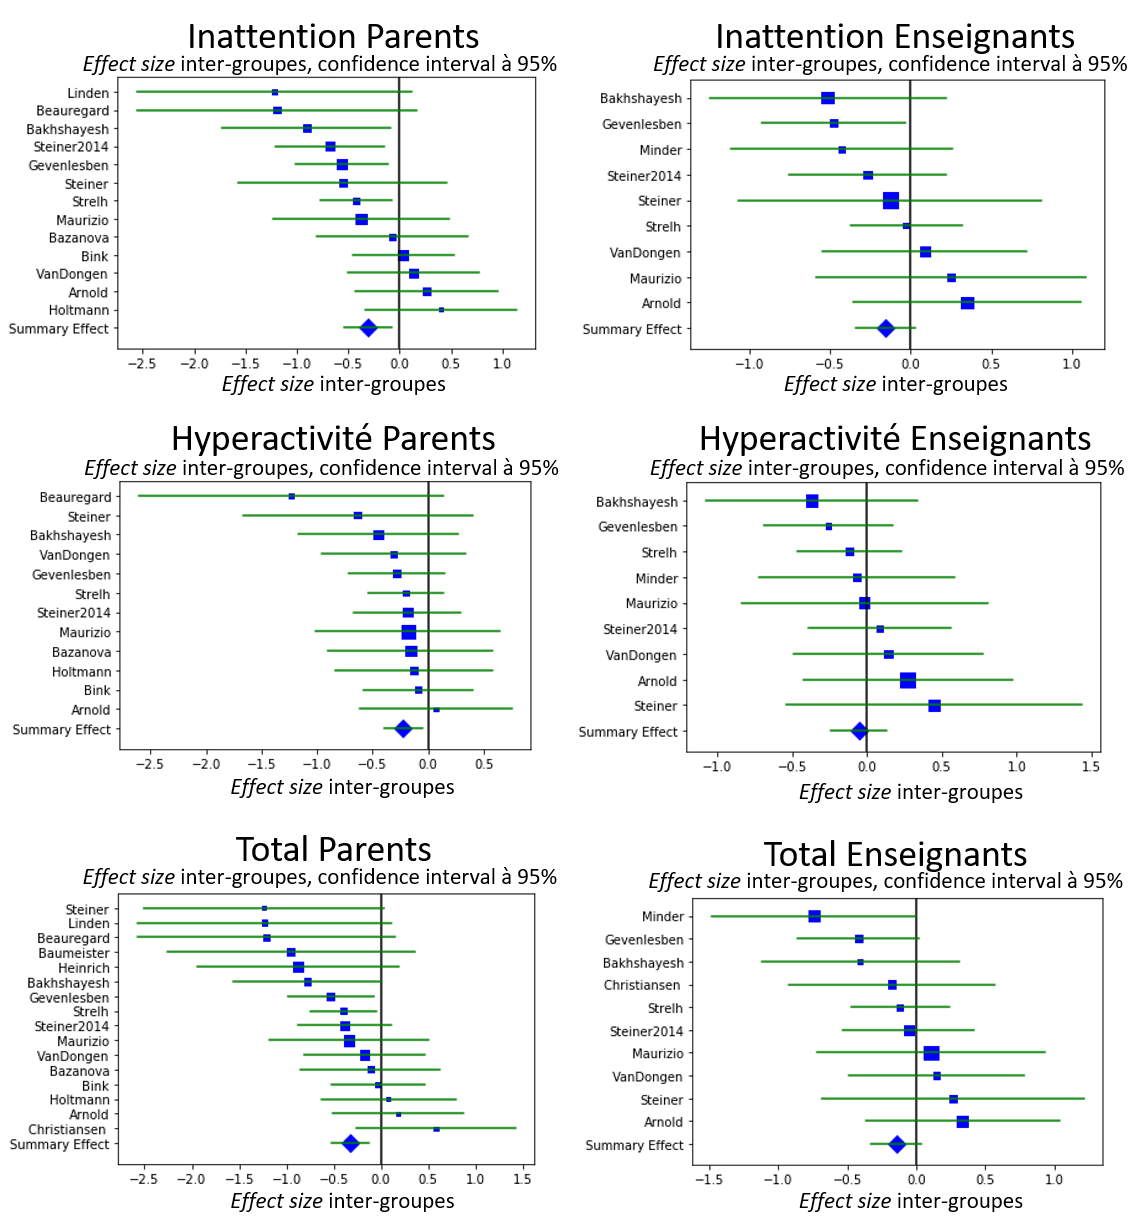
\includegraphics[width=1\linewidth]{figures/chapter-2/meta-analysis-forest-plots} 
  \caption[\textit{Forest plots} de la mise à jour de \citet{Cortese2016}.]{\textit{Forest plots} des \gls{es}-inter-groupes (les carrés bleus) avec 
	leur intervalle de confiance à 95\% (en vert) obtenus après la mise à jour de 
	\citet{Cortese2016}. Le losange bleu correspond à l'\gls{est}.
	Un \gls{es}-inter-groupes négatif est en faveur du \gls{nfb}.}
  \label{Figure:meta_analysis_forest_plots}
\end{figure}

Afin de détecter un biais de publication, une hétérogénéité parmi les études incluses ou la faible qualité méthodologique de certaines études, 
deux \textit{funnel plot} basés sur les \gls{es}-inter-groupes calculés sur les évaluations des symptômes totaux par les parents et les enseignants sont 
tracés à la Figure~\ref{Figure:meta_analysis_funnel_plots}. 

\begin{figure}[h!]
  \centering
	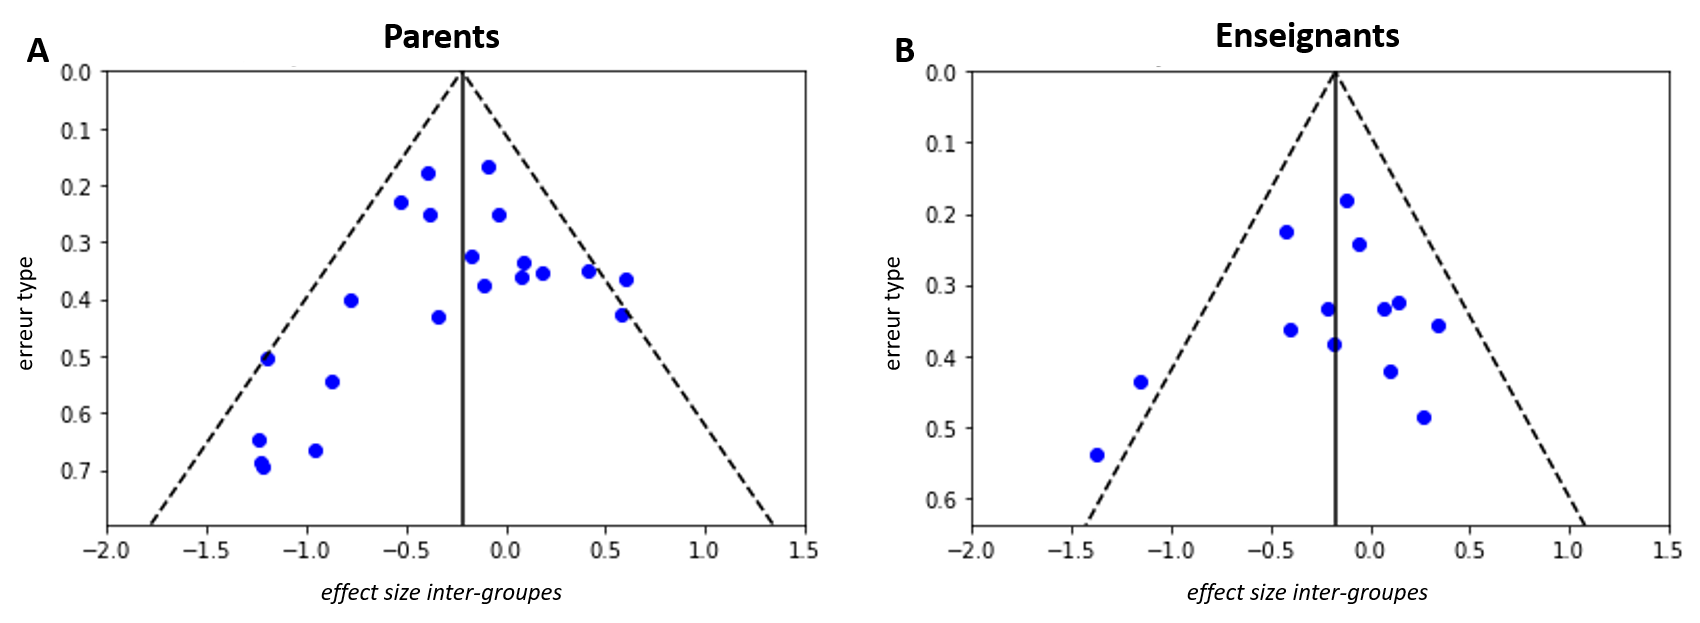
\includegraphics[width=1\linewidth]{figures/chapter-2/meta-analysis-funnel-plots} 
  \caption[\textit{Funnel plots} de la mise à jour de \citet{Cortese2016}.]{\textit{Funnel plots} obtenus pour les \gls{es}-inter-groupes calculés 
	sur les évaluations des symptômes totaux par les parents (en \textbf{A}) et 
	les enseignants (en \textbf{B}) avec un intervalle de confiance à 95\%.}
  \label{Figure:meta_analysis_funnel_plots}
\end{figure}

Visuellement, alors que le \textit{funnel plot} correspondant aux \gls{est} des enseignants semble plutôt symétrique, celui des parents parait asymétrique. 
Pour plus de précision, le test d'Egger a également été utilisé pour déterminer statistiquement si un biais s'est glissé dans l'analyse \citep{Egger1997} :
\begin{description}
\item[pour les parents :] contrairement à ce qui est observé, le \textit{funnel plot} n'est pas asymétrique, l'\textit{intercept} ne diffère pas 
significativement de 0 ($p$-value = 0.264),
\item[pour les enseignants :]  le \textit{funnel plot} n'est pas non plus asymétrique ($p$-value = 0.543).
\end{description}

Les études en dehors des pseudo limites de confiance à 95\% de l'\gls{est} sous le modèle à effet fixe sont : 
\begin{itemize}
\item pour les parents : \citet{Christiansen2014}, 
\item pour les enseignants : \citet{Moreno2019, Shereena2019}. 
\end{itemize}
 
\subsubsection{Résultats de la mise à jour sur les sous-groupes}
 
En ce qui concerne le sous-groupe \emph{protocole standard}, seul l'\gls{est} de la composante totale évaluée par les parents est significatif ($p$-value = 0.047). 
L'\gls{est} calculé pour la composante totale évaluée par les enseignants est limite significatif ($p$-value = 0.053).

Le sous-groupe \emph{pas de traitement médicamenteux en simultané} ne présente que l'\gls{est} de la composante inattention évaluée par les parents de 
significatif ($p$-value = 0.017).

\section{Discussion} 

Les méta-analyses doivent être menées rigoureusement, ainsi pour guider les auteurs des recommandations existent comme celles de PRISMA \citep{Moher2009}.
La réplication et la mise à jour présentées ici remplissent la majorité des points de cette \textit{checklist}, sauf notamment l'évaluation du risque de biais dans chaque étude.
Par ailleurs, elles ont été effectuées avec le package Python dont la fiabilité n'a été testée que sur une méta-analyse.
 
Le travail décrit précédemment a pour but d'explorer l'impact de certains choix de \citet{Cortese2016} qui ont été débattus dans la communauté scientifique 
\citep{Micoulaud2016}. Nous résumons ici la liste des changements, leur justification et leurs conséquences sur les résultats puis mettons en évidence 
les contributions de la mise à jour de la méta-analyse. 

\subsection{Discussion sur les résultats obtenus} \label{replication_and_update}

Les résultats obtenus suite à la réplication et à la mise à jour de \citet{Cortese2016} sont analysés et mis en perspective avec la littérature existante.

\subsubsection{Réplication}

Un des choix qui a été fait ici est d'utiliser la Conners-3 Teachers \citep{Conners2008} plutôt que la BOSS Classroom \citep{Shapiro2010} 
pour calculer les \gls{es}-inter-groupes obtenus par les évaluations des enseignants du fait de son utilisation plus commune \citep{Christiansen2014, Bluschke2016}.
Toutefois, l'utilisation de l'une ou l'autre de ces échelles ne change pas la significativité statistique des \gls{est} calculés pour les enseignants. 

La seconde différence entre \citep{Cortese2016} et la réplication effectuée ici est que le calcul des \gls{es}-inter-groupes de \citet{Arnold2014} se base 
sur les valeurs à post-test obtenues après 40 sessions de \gls{nfb} au lieu de valeurs temporaires obtenues après 12 sessions. Des études montrent
que le nombre de sessions est corrélé positivement avec les changements observés sur l'\gls{eeg} \citep{Vernon2004}, ainsi un faible nombre de sessions mènerait
à des \gls{es}-inter-groupes plus petits. Or, ici étonnamment les \gls{es}-inter-groupes calculés après la réalisation de toutes les sessions sont plus faibles que ceux 
obtenus après 12 sessions, ce qui n'est pas favorable à l'efficacité du \gls{nfb}. Toutefois, ces différences ne changent pas la significativité statistique des \gls{est}. 

En conclusion, sur la base de cette étude de sensibilité, nous suggérons que les points de débat soulevés par \citet{Micoulaud2016} ne sont pas majeurs 
quant à l'analyse et l'interprétation des résultats obtenus.

\subsubsection{Mise à jour} \label{meta_analysis_update}

La méta-analyse de \citep{Cortese2016} a déjà fait l'objet d'une mise à jour présentée dans \citet{Bussalb2019clinical} qui a intégré les études de 
\citep{Bazanova2018, Baumeister2016} et \citet{Strehl2017}. Cette mise à jour confirmait les résultats de \citep{Cortese2016} : les \gls{est} calculés 
à partir des évaluations des parents sont en faveur de l'efficacité du \gls{nfb}, au contraire des évaluations des enseignants. 

Les résultats obtenus ici sont globalement les mêmes qu'après la mise à jour de \citet{Bussalb2019clinical} au niveau de la significativité statistique : la seule
différence importante est la perte de la significativité statistique de l'\gls{est} pour la composante hyperactivité évaluée par les parents ($p$-value = 0.069).
Les \gls{est} évalués par les enseignants sont, quant à eux, toujours non significatifs ($p$-value pour la composante totale =  0.09). 

Cette mise à jour conduit à des \gls{est} plus faibles en valeur absolue que ceux obtenus par \citet{Cortese2016} comme l'illustrent les \textit{forest plots} à 
la Figure~\ref{Figure:meta_analysis_forest_plots} : par exemple l'\gls{est} calculé pour la composante totale évaluée par les parents est de -0.23 alors
que la réplication de \citet{Cortese2016} résumée à la Table~\ref{Table:table_meta_review_comparison_replication_cortese} menait à un \gls{est} de -0.32.

La détection de biais dans cette mise à jour s'est déroulée en deux temps : une analyse visuelle des \textit{funnel plots} présentés à la Figure~\ref{Figure:meta_analysis_funnel_plots}
puis le test d'Egger. Aucun biais ne s'est immiscé dans les évaluations des enseignants ($p$-value du test d'Egger = 0.543) contrairement à ce qu'avaient trouvé \citet{Cortese2016} ($p$-value = 0.042). 
\citet{Cortese2016} avaient expliqué ce résultat non pas par la présence d'un biais de publication, mais par le fait que les plus petites études sont 
de moins bonne qualité et donc n'arrivent pas à montrer l'efficacité du \gls{nfb}. En effet, en cas de biais de publication, les résultats des petites
études auraient été en faveur du \gls{nfb}. 

En ce qui concerne les évaluations des parents, le \textit{funnel plot} parait asymétrique, or le test d'Egger contredit cette observation ($p$-value = 0.264). 
Cela pourrait s'expliquer par le faible poids associé aux études qui causent cette asymétrie visuelle. 

Enfin, l'ajout de ces sept nouvelles études donne plus de puissance statistique aux résultats, notamment pour l'analyse des sous-groupes menée par \citet{Cortese2016}.

En effet, pour la sous population suivant un protocole \gls{nfb} standard \citep{Arns2014}, \citet{Cortese2016} avaient noté que les \gls{pblind} observaient
une différence statistiquement significative entre le \gls{nfb} et les groupes contrôles en faveur du \gls{nfb}. Alors que cette tendance a été confirmée avec l'ajout 
de \citet{Baumeister2016} et \citet{Strehl2017} dans \citet{Bussalb2019clinical}, la mise à jour présentée ici rend presque tous les \gls{est} initialement significatifs 
non significatifs ; désormais seul l'\gls{est} de la composante totale évaluée par les parents l'est encore ($p$-value = 0.047). 
L'\gls{est} calculé pour la composante totale évaluée par les enseignants est limite significatif ($p$-value = 0.053). Ces résultats remettent en question l'efficacité
supérieure des protocoles standards.

En ce qui concerne le sous-groupe constitué d'études qui interdisent la prise de médicaments, la seule différence avec \citep{Cortese2016} est la perte de   
significativité statistique de l'\gls{est} de la composante hyperactivité évaluée par les parents ($p$-value = 0.062).

\subsection{Hétérogénéité des études} 

Même si les méta-analyses regroupent les études répondant toutes aux critères d'inclusion comme, par exemple, ceux énoncés à \ref{selection_studies}, 
elles diffèrent tout de même sur de nombreux points, comme le nombre de sessions et la durée du traitement, limitant la fiabilité de leurs résultats 
comme le soulignent \citet{Alkoby2017}. Afin de pallier 
cette hétérogénéité, l'analyse peut cibler une population plus précise, comme ce qui a été effectué lors de l'analyse
des sous populations. Cependant, ce genre de restriction souffre d'une puissance statistique plus faible et regroupe encore des études fortement hétérogènes.
En effet, même si seuls les protocoles \gls{scp}, \gls{tbr} et \gls{smr} sont utilisés, ils restent intrinsèquement différents et il est probable que leur
efficacité ne soit pas la même. 

Par ailleurs, le matériel d'acquisition utilisé, ainsi que le traitement du signal varient d'une étude à l'autre, or ces points sont sans doute centraux 
dans la performance du traitement. 

De plus, aucun consensus n'existe quant au nombre de sessions ou à la durée du traitement, ainsi ces choix sont très variables d'une étude à l'autre et peu
souvent questionnés, bien qu'ils soient centraux dans la théorie de l'apprentissage.

\section{Importance de la mise à jour des méta-analyses} \label{need_to_update_meta_analysis}

Afin d'éviter de tomber dans le \textit{p-hacking}, c'est à dire faire en sorte d'obtenir un résultat significatif, il est important de ne pas arrêter la collecte de données 
et donc de figer les résultats une fois que la $p$-value de l'\gls{est} passe sous le seuil de significativité de 0.05 \citep{Head2015, Coffman2015}. En effet, l'arrêt prématuré des résultats peut
générer un biais : par exemple la $p$-value peut être significative à un instant $t$ avec un certain nombre de sujets inclus, puis perdre sa significativité statistique à
$t + 1$ et ne plus la retrouver. Ces deux configurations sont représentées avec des données factices à la Figure~\ref{Figure:meta-analysis-evolution-p-value-examples}.

\begin{figure}[h!]
  \centering
	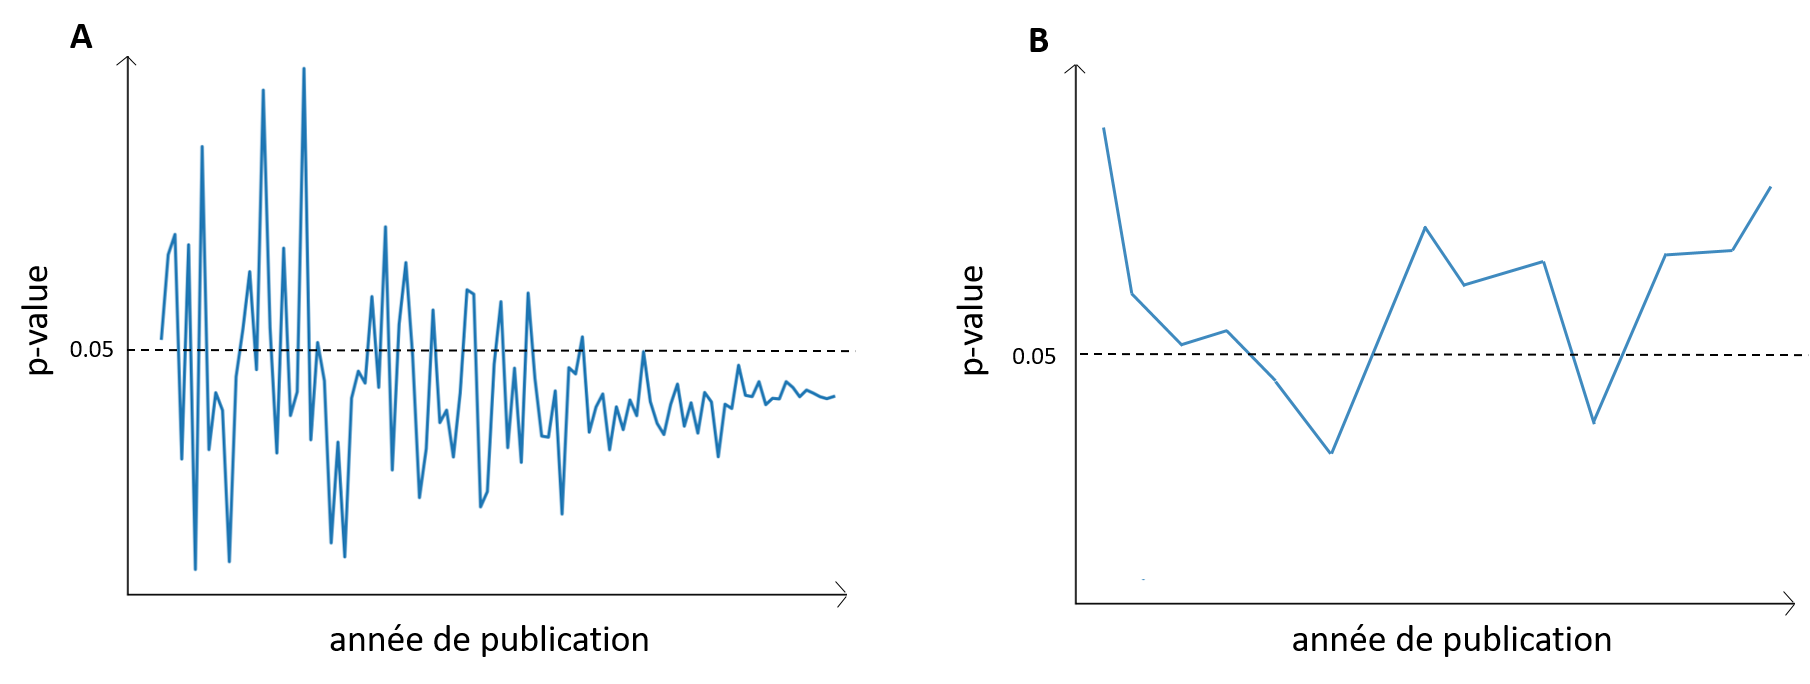
\includegraphics[width=1\linewidth]{figures/chapter-2/meta-analysis-evolution-p-value-examples} 
  \caption[Exemples d'évolution des $p$-value d'\gls{est} factices au fur et à mesure que la taille de l'échantillon augmente.]
	{Exemples d'évolution des $p$-value d'\gls{est} factices au fur et à mesure que la taille de l'échantillon augmente. 
	En \textbf{A}, la $p$-value se stabilise visuellement sous le seuil de significativité statistique suite à l'ajout de nouveaux sujets ; en \textbf{B}, la $p$-value 
	passe temporairement sous le seuil de significativité puis s'en éloigne suite à l'ajout de nouveaux sujets. 
	Le seuil de significativité statistique à 5\% est représenté en pointillés noirs.}
  \label{Figure:meta-analysis-evolution-p-value-examples}
\end{figure}

Les conclusions d'une méta-analyse pourraient donc souffrir de l'arrêt prématuré des analyses lorsque la $p$-value de l'\gls{est} n'est pas stable. 
Ainsi, la méta-analyse de \citet{Cortese2016} a déjà fait l'objet de deux mises à jour, dont les différences vont être comparées par la suite : 
la première a été publiée en 2019 \citep{Bussalb2019clinical} et la deuxième est présentée en \ref{selection_studies}. 

\subsection{Mise en évidence de l'importance des mises à jour} \label{methods_importance_to_update_meta_analysis}

L'importance de mettre à jour les méta-analyses est étudiée en deux temps :
\begin{itemize}
\item par l'évolution de l'\gls{est} calculé sur la composante totale au fur et à mesure de l'inclusion des études selon leur année de publication ; l'intervalle de confiance à 95\% est 
aussi représenté,
\item par l'évolution de la $p$-value de ces \gls{est} ; l'intervalle de confiance à 95\% des $p$-values
est obtenu avec les $p$-values de chaque étude incluse. Une fois cet intervalle, noté CI, obtenu, ses bornes sont ajustées de façon à prendre en compte le fait 
que la $p$-value est une valeur bornée entre 0 et 1 \citep{Mandelkern2002} : 
\begin{equation}
\label{eq:metareview_confidence_interval_evolitio_p_value}
\text{CI} = \begin{cases}
           [max(0;\text{borne inférieure}) ; max(0;\text{borne supérieure})], \\
					 [min(1;\text{borne inférieure}) ; min(1;\text{borne supérieure})].
					  \end{cases}
\end{equation}
\end{itemize}

L'évolution des \gls{est} est considérée comme stable lorsque visuellement elle semble converger. Quant à l'évolution des $p$-values, elle est
estimée stable lorsque les bornes de son intervalle de confiance sont au-dessus (ou en-dessous) du seuil de significativité à 5\%.

Les courbes sont tracées pour les évaluations des parents (\gls{mprox}) et des enseignants (\gls{pblind}). Le nombre de sujets par étude (NS) et cumulatif (NSC) sont précisés sur les axes 
des abscisses en haut de chaque graphique. Les NSC sont obtenus de la façon suivante : $\text{NSC}(k) = \text{NSC}(k - 1) + \text{NS}(k)$, avec $k$ l'indice de l'étude incluse
allant de $1$ à $K$, avec $K$ le nombre total d'études incluses.
 
Par ailleurs, la réplication de la méta-analyse de \citet{Cortese2016} ainsi que ses mises
à jour sont symbolisées sur les tracés par une étoile si l'\gls{est} est statistiquement significatif ou par un carreau sinon : les symboles
rouges correspondent aux résultats de la réplication de \citet{Cortese2016} (cf. \ref{replication}), les verts à ceux de \citet{Bussalb2019clinical} et les violets à ceux de la mise à jour décrite en \ref{selection_studies}. Les méta-analyses
étant généralement publiées quelque temps après la fin de la sélection des études, leur année de publication est représentée grâce à un point de la même couleur que le carreau ou
l'étoile relié au résultat de la méta-analyse par une droite en pointillés. 

L'axe des ordonnées a été inversé de façon à ce que les points en hauteur correspondent aux méta-analyses les plus favorables au traitement.

Tous les \gls{est} obtenus ont été calculés à l'aide du package Python développé pour mener les analyses décrites dans ce chapitre
\citep{Bussalb2019clinical} et avec les choix qui ont été faits lors la réplication de la méta-analyse de \citet{Cortese2016} présentée en \ref{replication}.


\subsection{Analyse des courbes de l'évolution de la taille d'effet totale}

La Figure~\ref{Figure:meta_analysis_evolution_est_total} représente l'évolution de l'\gls{est} calculé grâce aux évaluations des parents (en \textbf{A}) et des 
enseignants (en \textbf{B}) sur la composante totale en fonction de l'année de publication des études satisfaisant le critère d'inclusion établi par \citep{Cortese2016} et énoncé en 
\ref{selection_studies}.

\begin{figure}[t]
  \centering
	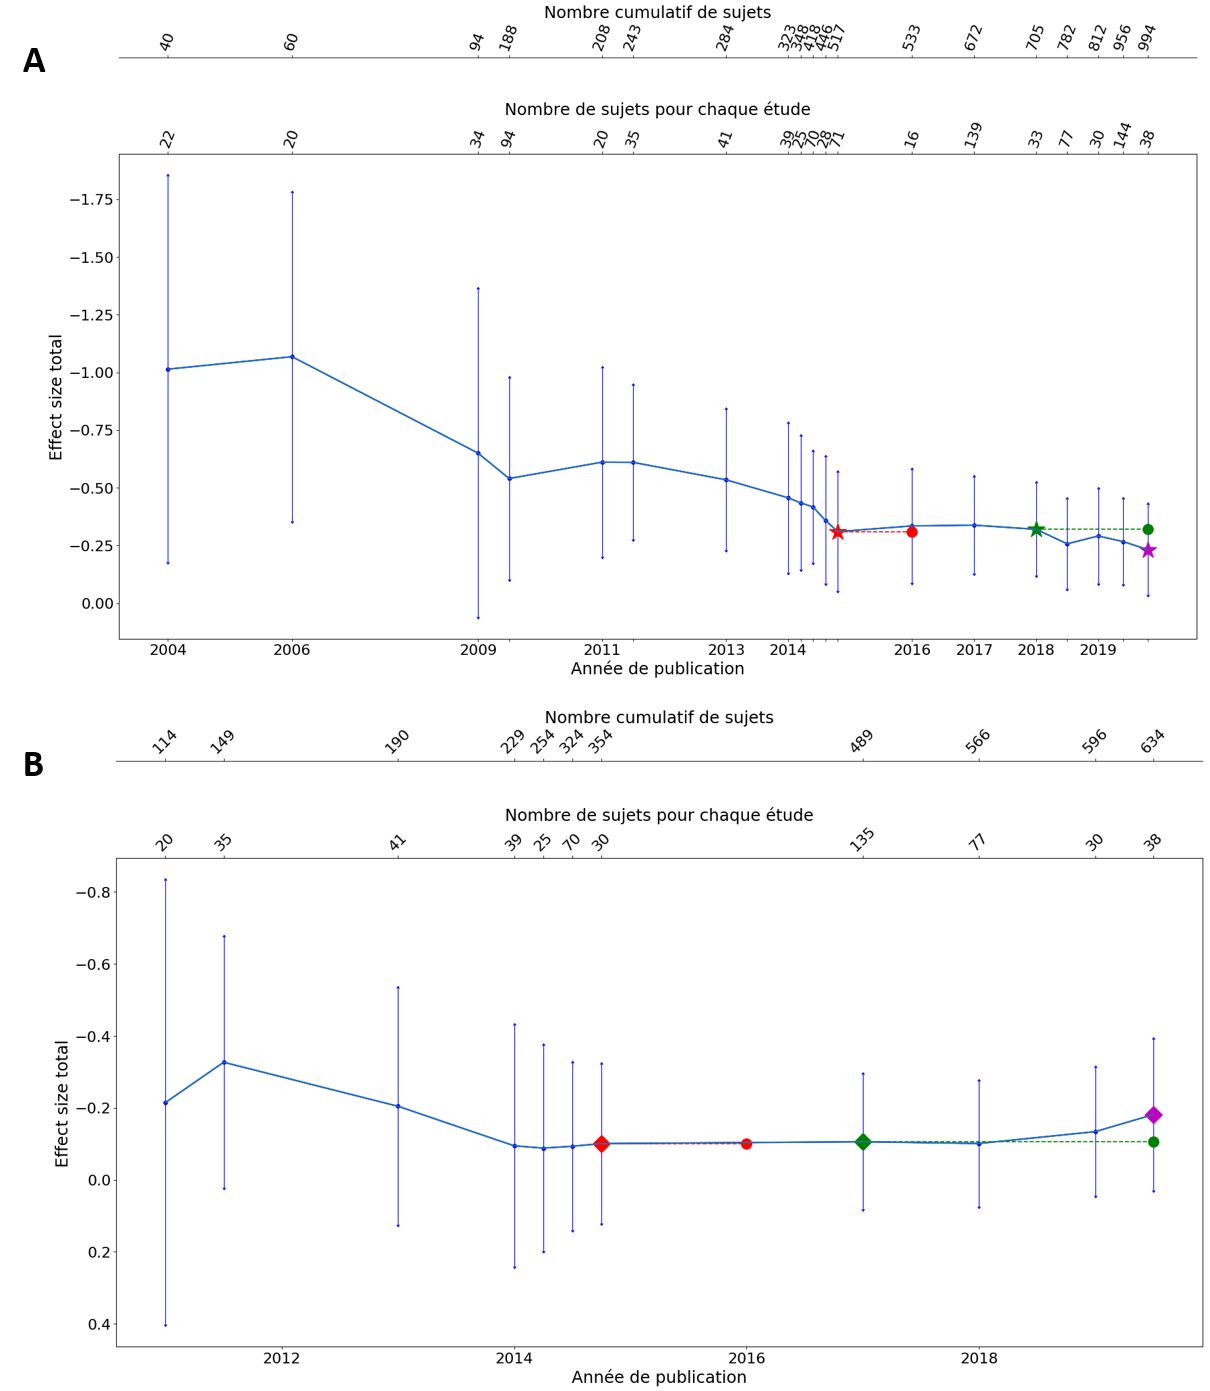
\includegraphics[width=1\linewidth]{figures/chapter-2/meta-analysis-evolution-summary-effect-total} 
  \caption[Evolution des \gls{est} au fur et à mesure de l'ajout de nouvelles études.]{Evolution des \gls{est} et de leur intervalle de confiance à 95\% au fur et à mesure de l'ajout des études satisfaisant le critère d'inclusion de \citet{Cortese2016} pour les évaluations des 
	parents en \textbf{A} et des enseignants en \textbf{B} sur la composante totale.
  Les résultats de la réplication de \citet{Cortese2016} sont représentés par des symboles rouges, ceux de \citet{Bussalb2019clinical} en vert et ceux présentés en \ref{selection_studies} en violet. Les étoiles 
	indiquent un \gls{est} statistiquement significatif, un losange un \gls{est} non statistiquement significatif. L'année de publication de ces méta-analyses est représentée grâce à un point de la couleur 
	d'intérêt relié au résultat de la méta-analyse par une droite en pointillés.
	Plus la valeur absolue de l'\gls{est} est élevée plus le traitement est efficace.
	Le nombre de sujets inclus par étude et cumulatif est indiqué sur les axes des abscissses supérieurs. La manière dont est calculé ce dernier est 
	décrite en \ref{methods_importance_to_update_meta_analysis}}
  \label{Figure:meta_analysis_evolution_est_total}
\end{figure}

Les \gls{est} obtenus grâce aux évaluations des parents (\textbf{A} de la Figure~\ref{Figure:meta_analysis_evolution_est_total}) varient de façon 
importante lorsque peu d'études sont incluses notamment entre 2006 et 2009, puis commencent à se stabiliser à 
partir de 2015, même si la valeur absolue des \gls{est} continue à diminuer. Les intervalles de confiance soulignent également cette stabilisation : ils diminuent 
avec l'augmentation du nombre d'études incluses. 

Cette tendance est également visible du côté des enseignants (\textbf{B} de la Figure~\ref{Figure:meta_analysis_evolution_est_total}). Toutefois, à partir 
de fin 2018 la valeur absolue des \gls{est} augmente.

Les mêmes graphiques sont tracés à la Figure~\ref{Figure:meta_analysis_evolution_est_std} mais cette fois en incluant seulement 
les études suivant un protocole standard \citep{Arns2014}.

\begin{figure}[t]
  \centering
	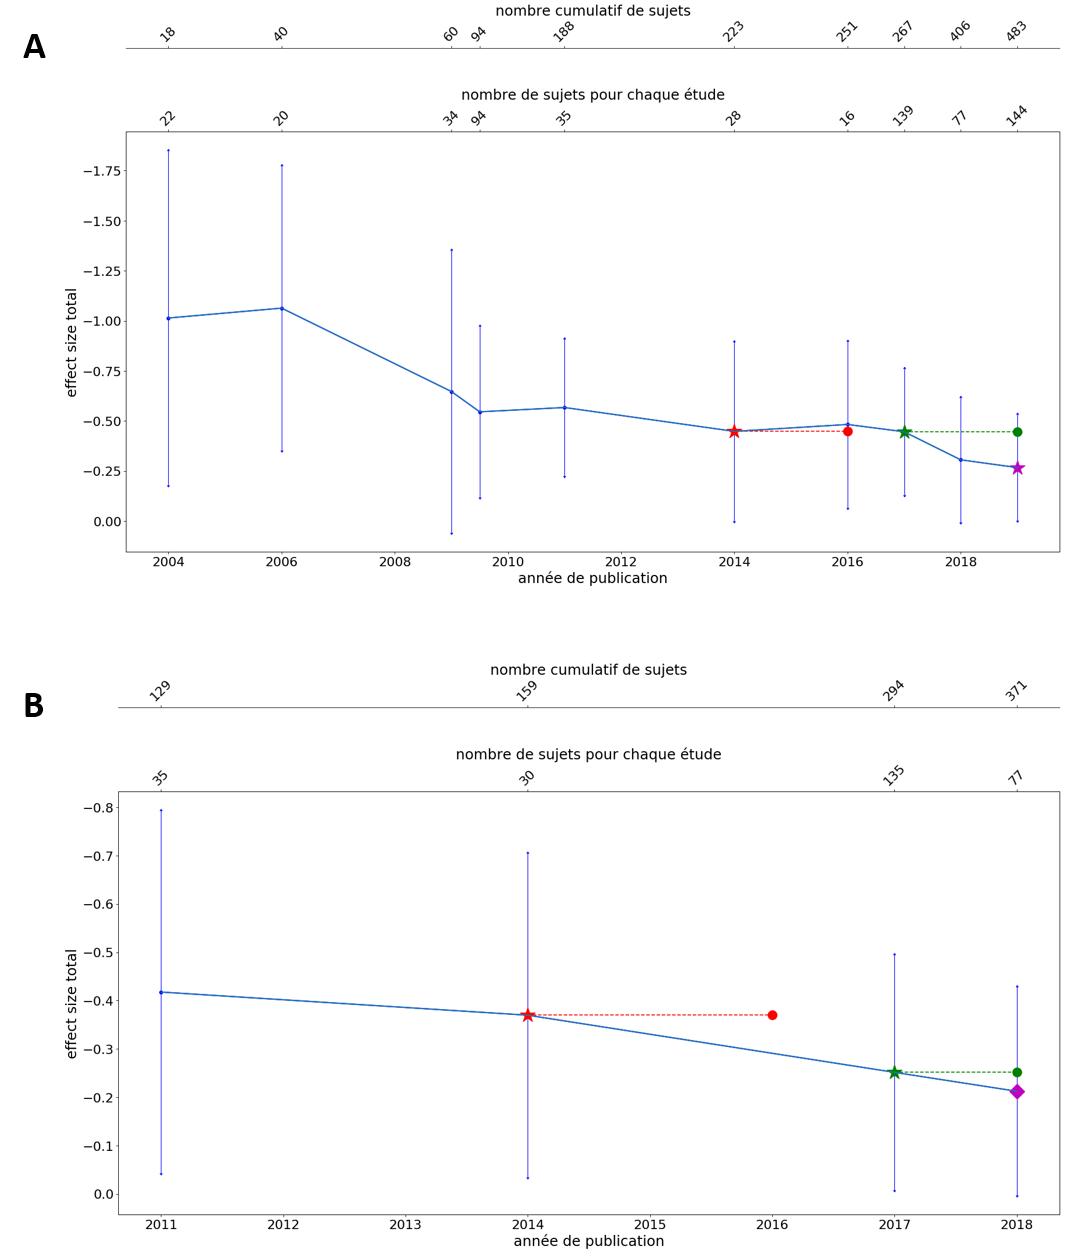
\includegraphics[width=1\linewidth]{figures/chapter-2/meta-analysis-evolution-summary-effect-std} 
  \caption[Evolution des \gls{est} au fur et à mesure de l'ajout de nouvelles études suivant un protocole standard.]{Evolution des \gls{est} et de leur 
	intervalle de confiance à 95\% au fur et à mesure de l'ajout des études suivant un protocole standard pour les évaluations des 
	parents en \textbf{A} et des enseignants en \textbf{B} sur la composante totale.
  Les résultats de la réplication de \citet{Cortese2016} sont représentés par des symboles rouges, ceux de \citet{Bussalb2019clinical} en vert et ceux présentés en \ref{selection_studies} en violet. Les étoiles 
	indiquent un \gls{est} statistiquement significatif, un losange un \gls{est} non statistiquement significatif. L'année de publication de ces méta-analyses est représentée grâce à un point de la couleur 
	d'intérêt relié au résultat de la méta-analyse par une droite en pointillés.
	Plus la valeur absolue de l'\gls{est} est élevée plus le traitement est efficace.
	Le nombre de sujets inclus par étude et cumulatif est indiqué sur les axes des abscissses supérieurs. La manière dont est calculé ce dernier est 
	décrite en \ref{methods_importance_to_update_meta_analysis}}
  \label{Figure:meta_analysis_evolution_est_std}
\end{figure}

\clearpage

Dans le cas des études satisfaisant la définition du protocole standard, les \gls{est} calculés à partir des évaluations des parents 
(\textbf{A} de la Figure~\ref{Figure:meta_analysis_evolution_est_std}) diminuent avec le temps, tout comme leur intervalle de confiance à 95\%. 
En ce qui concerne les \gls{est} obtenus grâce aux enseignants (\textbf{B} de la Figure~\ref{Figure:meta_analysis_evolution_est_std}), un faible nombre d'études 
est inclus et, alors que dans les cas précédents la diminution de l'\gls{est}ne menait pas à une perte de significativité statistique parmi les méta-analyses, 
ici la mise à jour de \citet{Cortese2016} présentée en \ref{selection_studies} conduit à un \gls{est} non significativement en faveur du \gls{nfb}. 

\subsection{Analyse des courbes de l'évolution de la $p$-value des tailles d'effet totales}

L'évolution des $p$-value de ces \gls{est} en fonction des études incluses est ensuite étudiée et présentée à la Figure~\ref{Figure:meta_analysis_evolution_pvalue_total} pour 
l'intégralité des études et à la Figure~\ref{Figure:meta_analysis_evolution_pvalue_std} pour les études suivant un protocole standard \citep{Arns2014}.

\begin{figure}[t]
  \centering
	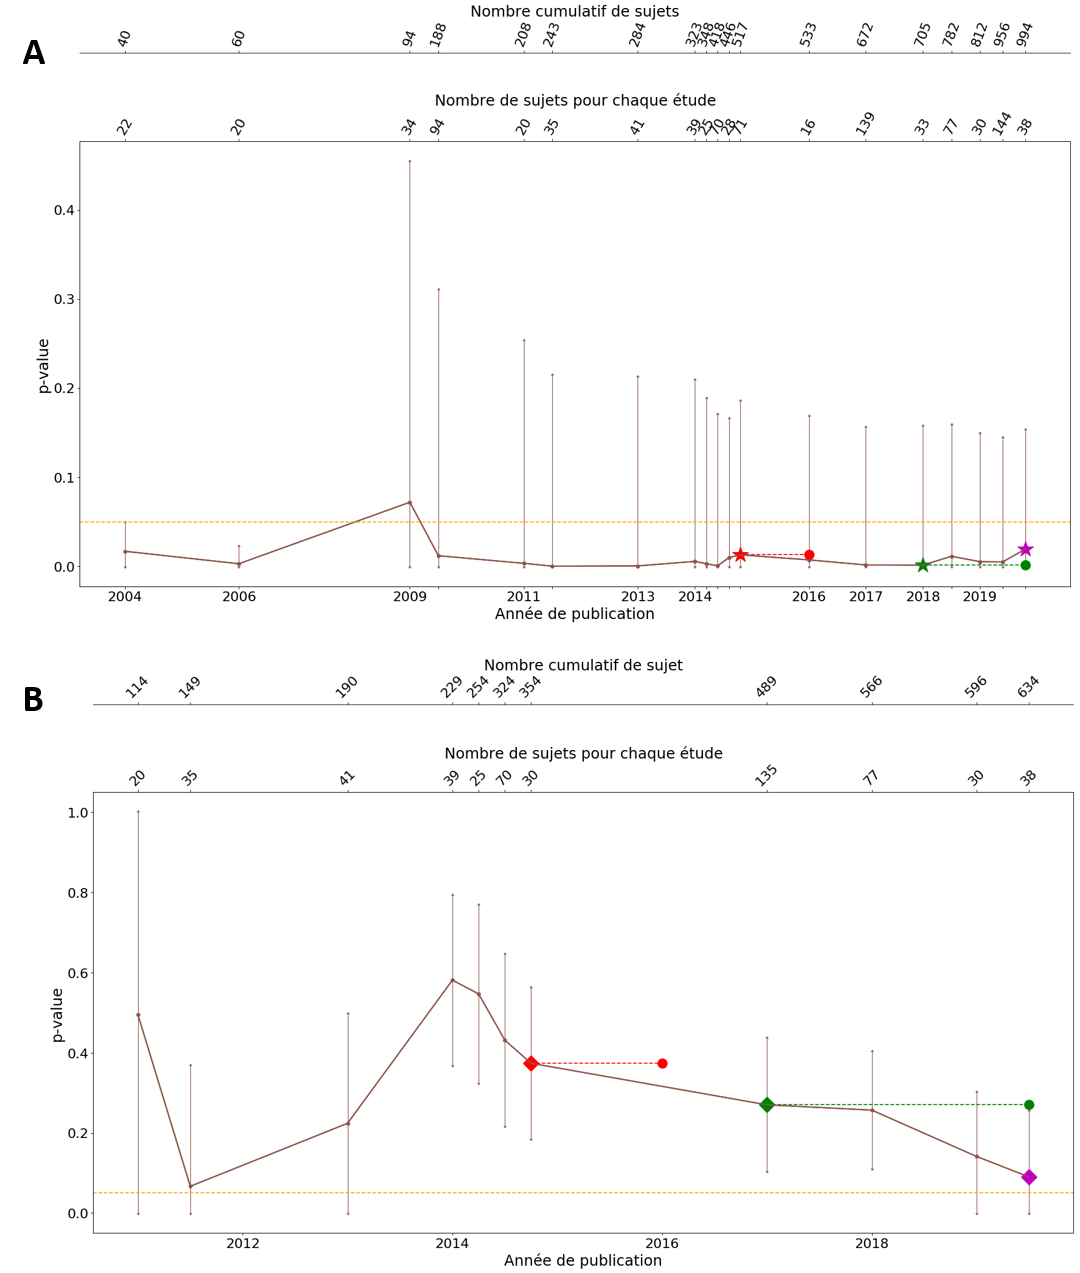
\includegraphics[width=1\linewidth]{figures/chapter-2/meta-analysis-evolution-pvalue-total} 
  \caption[Evolution de la $p$-value des \gls{est} au fur et à mesure de l'ajout de nouvelles études.]{Evolution de la $p$-value des \gls{est} et de leur intervalle de confiance à 95\% au fur et à mesure de l'ajout des études satisfaisant le critère d'inclusion de \citet{Cortese2016} pour les évaluations des 
	parents en \textbf{A} et des enseignants en \textbf{B} sur la composante totale.
  Les résultats de la réplication de \citet{Cortese2016} sont représentés par des symboles rouges, ceux de \citet{Bussalb2019clinical} en vert et ceux présentés en \ref{selection_studies} en violet. Les étoiles 
	indiquent un \gls{est} statistiquement significatif, un losange un \gls{est} non statistiquement significatif. L'année de publication de ces méta-analyses est représentée grâce à un point de la couleur 
	d'intérêt relié au résultat de la méta-analyse par une droite en pointillés.
	Le nombre de sujets inclus par étude et cumulatif est indiqué sur les axes des abscissses supérieurs. La manière dont est calculé ce dernier est 
	décrite en \ref{methods_importance_to_update_meta_analysis}
	Le seuil de significativité à 5\% est représenté par des pointillés orange.}
  \label{Figure:meta_analysis_evolution_pvalue_total}
\end{figure}

\begin{figure}[t]
  \centering
	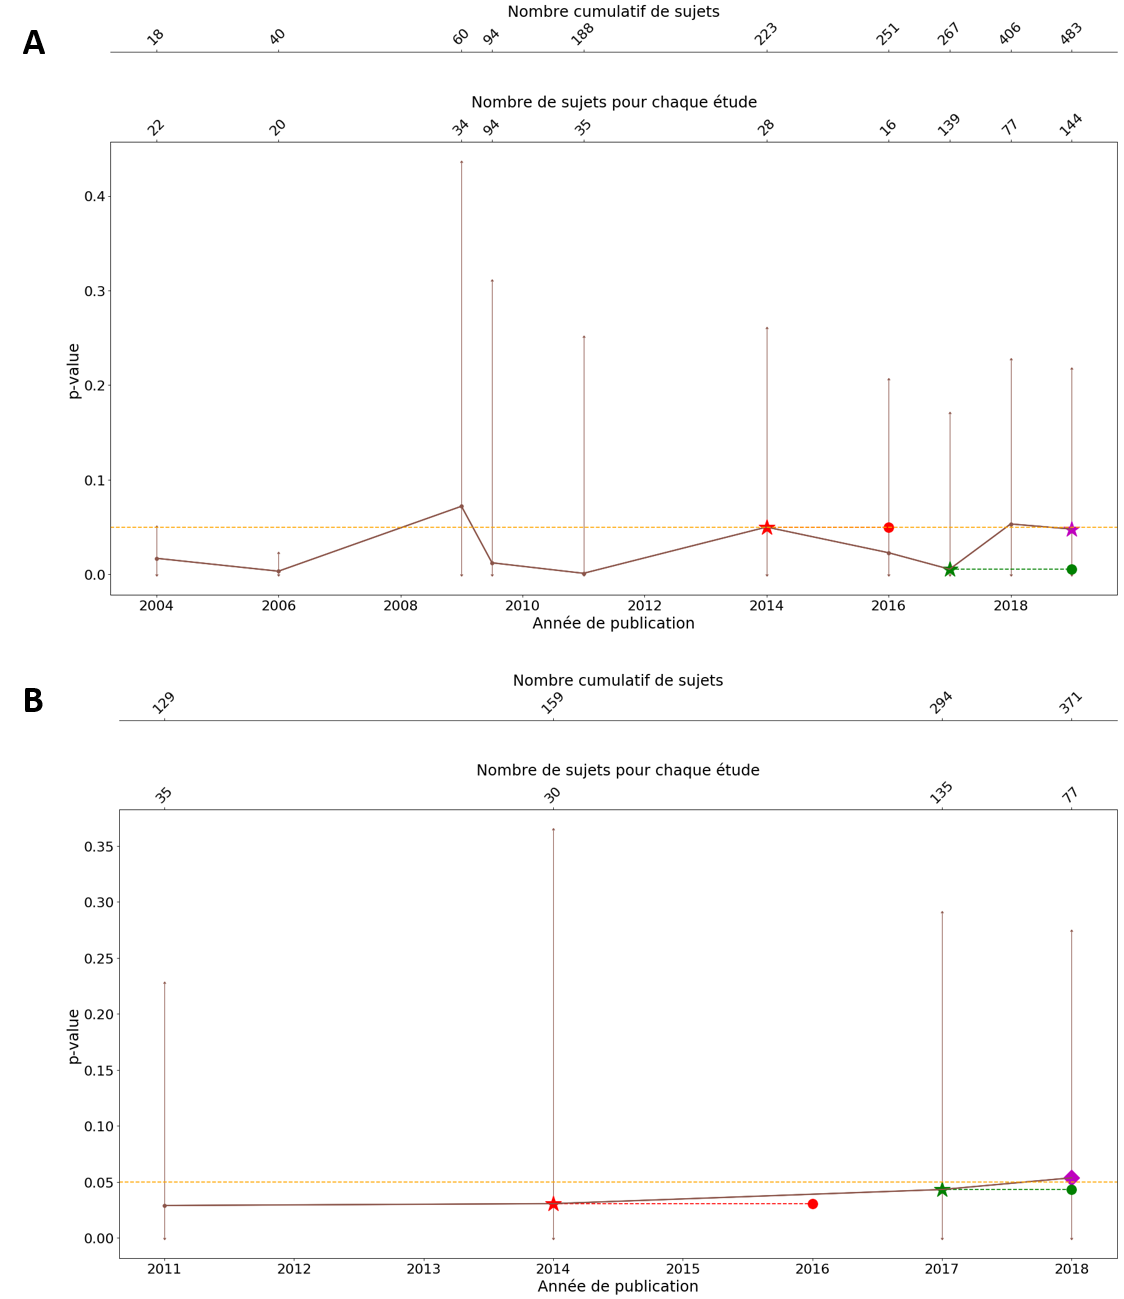
\includegraphics[width=1\linewidth]{figures/chapter-2/meta-analysis-evolution-pvalue-std} 
  \caption[Evolution de la $p$-value des \gls{est} au fur et à mesure de l'ajout de nouvelles études suivant un protocole standard.]{Evolution de la $p$-value 
	des \gls{est} et de leur intervalle de confiance à 95\% au fur et à mesure de l'ajout des études répondant à la définition du protocole standard pour les évaluations des 
	parents en \textbf{A} et des enseignants en \textbf{B} sur la composante totale.
  Les résultats de la réplication de \citet{Cortese2016} sont représentés par des symboles rouges, ceux de \citet{Bussalb2019clinical} en vert et ceux présentés en \ref{selection_studies} en violet. Les étoiles 
	indiquent un \gls{est} statistiquement significatif, un losange un \gls{est} non statistiquement significatif. L'année de publication de ces méta-analyses est représentée grâce à un point de la couleur 
	d'intérêt relié au résultat de la méta-analyse par une droite en pointillés.
	Le nombre de sujets inclus par étude et cumulatif est indiqué sur les axes des abscissses supérieurs. La manière dont est calculée ce dernier est 
	décrite en \ref{methods_importance_to_update_meta_analysis}.
	Le seuil de significativité à 5\% est représenté par des pointillés orange.}
  \label{Figure:meta_analysis_evolution_pvalue_std}
\end{figure}

\clearpage

Tout d'abord, en ce qui concerne l'évolution de la $p$-value en incluant l'intégralité des études pour les 
évaluations des parents (\textbf{A} de la Figure~\ref{Figure:meta_analysis_evolution_pvalue_total}), on remarque que les $p$-values sont toutes
en-dessous du seuil de significativité à 5\% sauf en 2009. Après 2009, les $p$-values varient moins et leur intervalle de confiance à 95\% diminue, 
ce qui laisse penser que nous sommes plutôt dans le cas \textbf{A} illustré à la Figure~\ref{Figure:meta-analysis-evolution-p-value-examples}. Toutefois,
la borne supérieure de l'intervalle de confiance n'est jamais en-dessous du seuil de significativité de 5\%.

Quant à l'évolution des $p$-values présentée en \textbf{B} de la Figure~\ref{Figure:meta_analysis_evolution_pvalue_total}, elle est
toujours non statistiquement significative, mais perd sa stabilité à partir de 2019.

Enfin, en ce qui concerne le groupe standard présenté à Figure~\ref{Figure:meta_analysis_evolution_pvalue_std}, les fluctuations des $p$-values 
sont moins importantes aussi bien pour les évaluations 
des parents (en \textbf{A}) que celles des enseignants (en \textbf{B}) mais restent instables. 
De plus, les $p$-values sont à la limite du seuil de significativité dans les deux cas lors de la dernière mise à jour.

\subsection{Discussion sur ces courbes}

Les courbes d'évolution des \gls{est} au fur et à mesure de l'inclusion de l'ensemble des études (Figure~\ref{Figure:meta_analysis_evolution_est_total}) 
illustrent le fait que l'\gls{est} 
devient visuellement de plus en plus stable avec le temps. Par ailleurs, la diminution des intervalles de confiance à 95\% montre que les résultats 
deviennent de plus en plus précis.

Les courbes correspondant à l'évolution de l'\gls{est} dans le sous-groupe des études suivant un protocole standard (Figure~\ref{Figure:meta_analysis_evolution_est_total}) 
fluctuent davantage du fait du nombre limité de sujets et d'études incluses.

Alors que les \gls{est} commencent dans l'ensemble à converger, leur $p$-value continue de fluctuer (Figure~\ref{Figure:meta_analysis_evolution_pvalue_total} et 
Figure~\ref{Figure:meta_analysis_evolution_pvalue_std}) même si sur la totalité des études elles s'accordent depuis 2011 sur la conclusion de \citet{Cortese2016} :
les évaluations des parents (\textbf{A} de la Figure~\ref{Figure:meta_analysis_evolution_pvalue_total}) sont significativement en faveur du \gls{nfb} 
au contraire des évaluations des enseignants (\textbf{B} de la Figure~\ref{Figure:meta_analysis_evolution_pvalue_total}). 
Toutefois, alors qu'elle était stable entre 2014 et 2018 pour les évaluations des enseignants, elle recommence à fluctuer à partir de 2019 : 
la $p$-value de la dernière mise à jour de \citet{Cortese2016} tend vers la significativité statistique, il serait donc intéressant 
de continuer à mettre à jour ce travail pour déterminer si cette $p$-value devient significative et le reste.

Dans le cas de l'évolution des $p$-values dans le sous-groupe des études suivant un protocole standard (Figure~\ref{Figure:meta_analysis_evolution_pvalue_std}), 
la dernière mise à jour 
de \citet{Cortese2016} conduit à des résultats limite significatifs pour les évaluations des parents (\textbf{A}) et à une perte de significativité statistique pour celles des 
enseignants (\textbf{B}), remettant en question les conclusions de \citet{Cortese2016} et \citet{Bussalb2019clinical} quant à l'efficacité des protocoles standards.
 
La $p$-value est très largement utilisée en méta-analyse, mais est également de plus en plus contestée du fait qu'elle soit trop souvent mal interprétée 
\citep{Halsey2019}. 
En effet, la $p$-value mesure le degré de compatibilité entre les données et l'hypothèse nulle, et non la probabilité que l'hypothèse nulle soit vraie

Ainsi, les chercheurs se tournent de plus en plus vers les statistiques bayésiennes, avec des outils comme le rapport de vraisemblance 
(\textit{likelihood ratio} en anglais) \citep{Dormuth2016}, ou le facteur de Bayes \citep{Morey2016, Rouder2011}. L'évolution de ces 
valeurs avec l'inclusion de nouvelles études serait intéressante à étudier. 

Pour conclure, la mise à jour des méta-analyses peut avoir une incidence sur la significativité statistique de la $p$-value, notamment dans le cas où peu d'études et donc de sujets
sont inclus. Continuer à inclure de nouvelles études permet d'augmenter la puissance statistque des calculs : en particulier les études les plus récentes sur l'efficacité du \gls{nfb}
appliqué aux enfants \gls{tdah} comportent de plus en plus de sujets.

Enfin, étant donné l'essor de l'utilisation du \gls{nfb} appliqué aux enfants \gls{tdah}, au moment de la publication d'une méta-analyse de nouvelles études satisfaisant ses critères d'inclusion
sont déjà disponibles comme illustré aux figures~\ref{Figure:meta_analysis_evolution_est_total} et ~\ref{Figure:meta_analysis_evolution_est_std}. Ainsi, à peine publiés, les résultats de la 
méta-analyse sont déjà obsolètes, ce qui appelle à leur mise à jour. 

Cette approche qui consiste à affiner les résultats à l'aide de nouvelles observations est l'une des bases de l'inférence bayésienne.

\section{Conclusion}

Cette partie s'est concentrée sur un outil couramment utilisé pour évaluer l'efficacité du \gls{nfb} : la méta-analyse. Ce travail a été l'occasion de mettre au point un package 
\textit{open-source} pour effectuer une méta-analyse en toute transparence et aider à la réplication ou à la mise à jour de ses résultats.

Ce package a justement été utilisé pour répliquer la méta-analyse de \citet{Cortese2016} dont certains points ont été discutés par la communauté scientifique. 
Il se trouve que les choix effectués par \citet{Cortese2016} s'avèrent anodins mais illustrent la complexité de l'émergence de la preuve
clinique.

Cette réplication a également mis en évidence l'importance de la disponibilité des données cliniques afin d'effectuer des calculs précis et de conclure de façon
plus fiable quant à l'efficacité d'un traitement. 

Il est important de noter qu'une méta-analyse ne rend compte de l'efficacité d'un traitement qu'à un moment donné : étant donné le nombre important d'études évaluant l'efficacité du \gls{nfb} 
pour les enfants souffrant du \gls{tdah}, mettre à jour les méta-analyses est nécessaire, c'est pourquoi un tel travail a été entrepris ici. Par ailleurs, l'analyse de l'évolution de l'\gls{est} et des $p$-values 
associées en fonction de l'ajout des études montrent que ces métriques tendent à se stabiliser depuis quelques années mais ne convergent pas encore, appelant à de nouvelles mises à jour.  

Les résultats des méta-analyses donnent une idée de l'efficacité du traitement étudié, même s'il faut garder à l'esprit que les études incluses
diffèrent sur différents points, ce qui est notamment vrai pour le \gls{nfb}. Afin de pallier cette faiblesse, des sous-groupes peuvent être étudiés comme ici avec le groupe d'études
suivant un protocole standard et celui d'études où les enfants ne prennent pas de médicaments.

Cependant cette approche ne gomme pas toutes les différences entre les études. Or, ces différences ont sans doute une influence sur l'efficacité du \gls{nfb}, ainsi nous proposons dans le chapitre 
suivant de tirer avantage de cette hétérogénéité entre les études pour tenter de mettre en évidence les facteurs 
techniques et/ou cliniques qui pourraient avoir une influence sur la performance du \gls{nfb}.

  